\documentclass[preprint,11pt]{elsarticle}
\usepackage{lmodern}
\usepackage{amsmath,amssymb,amsthm,booktabs}
\usepackage{needspace}
\usepackage{microtype}
\usepackage{tikz}
\usepackage{float}
\usepackage{graphicx}
\usetikzlibrary{arrows.meta,positioning}
\usepackage[hidelinks]{hyperref}
\usepackage[margin=1in]{geometry}
\raggedbottom
\renewcommand{\topfraction}{0.9}
\renewcommand{\bottomfraction}{0.8}
\renewcommand{\textfraction}{0.1}
\setlength{\textfloatsep}{14pt plus 2pt minus 2pt}
\setlength{\floatsep}{12pt plus 2pt minus 2pt}
\makeatletter
% Paragraph headings in this source already include their final punctuation.
\let\paragraph\elsparagraph
\setlength{\@fptop}{0pt}
\setlength{\@fpsep}{16pt}
\setlength{\@fpbot}{0pt plus 1fil}
\makeatother
\newtheorem{theorem}{Theorem}[section]
\newtheorem{lemma}[theorem]{Lemma}
\newtheorem{proposition}[theorem]{Proposition}
\newtheorem{corollary}[theorem]{Corollary}
\newtheorem{remark}[theorem]{Remark}
\newcommand{\norm}[1]{\lVert #1\rVert}
\newcommand{\ind}[1]{\mathbf{1}\{#1\}}
\journal{Neurocomputing}
\biboptions{sort&compress}
\hypersetup{pdftitle={Calibrating Normalized Hypergraph Spectral Risk under Node-Induced Dependence},
  pdfauthor={Shen Peng, Rui Wang, Yunchao He}}

\begin{document}
\begin{frontmatter}
\title{Calibrating Normalized Hypergraph Spectral Risk under Node-Induced Dependence}
\author[a]{Shen Peng\corref{corresponding}}
\ead{shen.peng23@student.xjtlu.edu.cn}
\author[a]{Rui Wang}
\author[a]{Yunchao He}
\cortext[corresponding]{Corresponding author.}
\address[a]{Academy of Artificial Intelligence and Advanced Technology,
Xi'an Jiaotong-Liverpool University, Suzhou 215412, China}

\begin{abstract}
Prediction-constructed hypergraphs couple incident relations through
shared node predictions, making edge marginals insufficient for spectral-risk
assessment. We connect normalized conditional influence, calibration under a
declared prediction law, and complete-run diagnostics. Conditional
expectations decompose the normalized operator into orthogonal node
responses and a remainder; a three-operator comparison separates fixed
degree weighting from dynamic normalization. On Cora-CC and DBLP-CA,
computed centered-norm ratios between node-induced and independent-edge
models decreased from 2.15--3.47 before normalization to 1.03--1.26
afterward, while a coherent controlled family reversed the comparison.
Under specified node laws at a 5\% target, node-calibrated native
exceedance means were 3.9\%--5.9\%, compared with 47.5\%--100\% for
independent-edge thresholds. With trained predictors, fitted node-product
thresholds instead yielded zero observed exceedances in the tested
settings. This conservative direction extended to NTU2012 and ModelNet40,
with zero exceedances in 200 evaluation runs per visual dataset;
independent-edge calibration yielded 26.5\% on ModelNet40. Complete-run
and split-sensitivity comparisons distinguish marginal rank validity
from the conditional behavior of a frozen threshold. A standard rank
argument supplies finite-sample validity under the declared exchangeable
score law. Together, the analysis and cross-domain comparisons identify
which joint dependence a calibration model must preserve and separate
the probability targets needed for upstream operator monitoring.
\end{abstract}
\begin{keyword}
Hypergraph learning \sep Relation estimation \sep Node influence \sep
Spectral fluctuation \sep Dependent errors \sep Risk calibration
\end{keyword}
\end{frontmatter}

\section{Introduction}\label{sec:intro}

Hypergraph learning aggregates information through group relations
\cite{feng2019hgnn,chien2022allset}. When predictions determine which
candidate relations are retained, one node prediction can change several
incident hyperedges at once. An independent-edge model can match every
retention probability while missing this joint variation. Risk assessment
must therefore specify how the predictions generating an operator vary.

Degree normalization introduces a second distinction. Matching the mean
raw relation operator does not generally match the mean normalized
operator, and raw fluctuation amplification need not survive
normalization. A third distinction arises with trained predictors:
sampling nodes independently from their estimated class frequencies
preserves their marginals but removes dependence induced by a shared
training run. These distinctions concern the same question:
\emph{how does node-induced dependence change normalized spectral risk,
and which prediction law must calibration preserve?}

We answer this question by connecting normalized conditional influence,
law-specific calibration, and repeated-run diagnostics. Conditional
expectations decompose the normalized operator into orthogonal
single-node influences and a remainder. A three-operator comparison then
distinguishes static degree weighting from dynamic normalization.
Keeping this mechanism analysis separate from monitoring permits a
standard finite-sample rank threshold with a precise probability target.
Finally, complete training runs test whether fitted node marginals
provide an adequate replacement law.

The contribution is this connection and its measured limits in
prediction-constructed hypergraphs. The conditional-expectation
decomposition and rank rule are established tools. Their application
shows why matching edge marginals, retaining node-induced dependence,
and retaining an entire training-run law are different requirements.
Experiments on controlled families, Cora-CC, and DBLP-CA evaluate these
requirements separately. Raw-operator amplification, cancellation, and
tail-risk results supply the mechanism foundation in
Appendices~\ref{sec:raw-mechanism} and~\ref{sec:raw-validation}; the
main analysis asks what remains true after normalization and calibration.

Finally, we extend the complete-run calibration protocol to two visual
object hypergraphs, NTU2012 and ModelNet40. These experiments test the
cross-domain behavior of fitted node-product and independent-edge
calibration, and distinguish marginal rank validity from the
conditional variability of a threshold estimated from finitely many
complete runs.

\subsection{Related work}
Matrix concentration controls independent matrix sums
\cite{tropp2012user} and matrix functions of independent variables
\cite{paulin2016efronstein}. Other dependence assumptions include
strong negative dependence and Markovian summands
\cite{amparore2025dependent,geuchen2024matrix}. Independence of node
coordinates does not imply independence of their induced edge events.
Our raw-operator comparison uses the classical ANOVA decomposition
\cite{hoeffding1948class}, related to overlap calculations for motif
counts \cite{matias2006motifs}; its normalized version retains the
conditional-expectation identity while changing the influences.
Decoupling \cite{delapena1999decoupling}, latent-position spectral
inference \cite{athreya2018statistical}, and hypergraph spectral
similarity \cite{hayhoe24spectral} address related operator questions
under their respective probability models.

Rank calibration uses exchangeability to control a new observation
jointly with the random calibration sample. This differs from requiring
the conditional error probability of every realized calibration sample
to equal a target \cite{vovk2012conditional}. Conformal risk control
extends split-conformal reasoning to expected monotone losses
\cite{angelopoulos2024crc}. We use the simpler scalar upper-tail rank
rule and prove its scope explicitly. The inference target is an
operator-deviation alarm under the declared law. Task-level performance
is a separate empirical outcome.

Structural-noise analysis and hyperedge refinement connect graph
reliability to learning performance
\cite{dong23structural,huang26trustworthy}. Here the learning task
motivates the relation construction, and spectral deviation under a
stated law serves as an upstream structural diagnostic. Its task-level
consequences require separate evaluation.

\section{Operators, Centers, and Prediction Laws}\label{sec:norm-model}

Fix a candidate hypergraph $E$ on $n$ nodes, with $|e|\ge2$.
For a prediction vector $Y$, define
\begin{equation}\label{eq:norm-operator}
\begin{aligned}
H_e&=\mathbf1_e\mathbf1_e^\top/|e|,&
a_e(Y)&=\ind{Y_u\text{ agree over }u\in e},\\
B(a)&=\sum_e a_eH_e,& A(a)&=B(a)+\kappa I,\\
D(a)&=\operatorname{diag}(A(a)\mathbf1),&
S(a)&=D(a)^{-1/2}A(a)D(a)^{-1/2}.
\end{aligned}
\end{equation}
The experiments use $\kappa=1$ and unit edge weights. Degrees are
recomputed for every draw: $d_v(a)=\kappa+\sum_{e\ni v}a_e$.
Thus $S(a)\sqrt{d(a)}=\sqrt{d(a)}$ and $\|S(a)\|_2=1$.
This is the specified nonnegative symmetric operator; an implementation
using another HGNN normalization requires its own definition.

Under an independent categorical node law $P[u,c]$, model A draws the
entire $Y$ and constructs every $a_e(Y)$. Model B draws edge slots
independently with probabilities
$p_e=\sum_c\prod_{u\in e}P[u,c]$. Duplicate node sets share an event
in A but are independent slots in this counterfactual B model.
Both arms have $\mathbb E B=\sum_ep_eH_e$. For the fixed-degree control,
\begin{equation}\label{eq:fixed-degree}
D_0=\operatorname{diag}((\mathbb E B+\kappa I)\mathbf1),\qquad
S_0(a)=D_0^{-1/2}(B(a)+\kappa I)D_0^{-1/2},
\end{equation}
the means still match by linearity. Generally
$\mathbb E_A S\ne\mathbb E_B S$, and
$S(p)\ne\mathbb E_A S$. We report their roles separately.

\paragraph{Mechanism and monitoring centers.}
Mechanism comparisons use each arm's own mean in
$\|S-\mathbb E_{\mathrm{arm}}S\|_2$, with independently estimated
means in the simulations. Monitoring uses one center $\widehat M$
estimated in an independent reference stage and then frozen:
\begin{equation}\label{eq:monitor-score}
T(Y)=\|S(a(Y))-\widehat M\|_2.
\end{equation}
Comparisons between calibrators use the same center and scoring
pipeline. The deterministic baseline $S(p)$ is used only for local
response analysis, not as an interchangeable estimate of $\mathbb E S$.

\paragraph{Three prediction-law levels.}
L1 specifies a known product law for node predictions and tests its
induced joint relation law. The synthetic error profiles use benchmark
labels to define this model; they are not estimates obtainable without
labels at deployment. L2 estimates node class frequencies in an
independent reference stage and resamples from their product. Its
validity within that fitted law does not establish validity for the
actual training process. L3 treats an entire prediction vector from
one training run as one observation. Exchangeability is required across
runs of the same protocol, rather than across nodes. Random labeled
sets, random training partitions, and initialization with a fixed
training set define separate L3 mechanisms.

Figure~\ref{fig:calibration-map} separates two parts of the analysis.
The operator chain isolates static degree weighting from dynamic degree
recomputation, while each prediction law supplies complete relation draws
to the same normalized scoring pipeline.
\Needspace{12cm}
\begin{figure}[H]
\centering
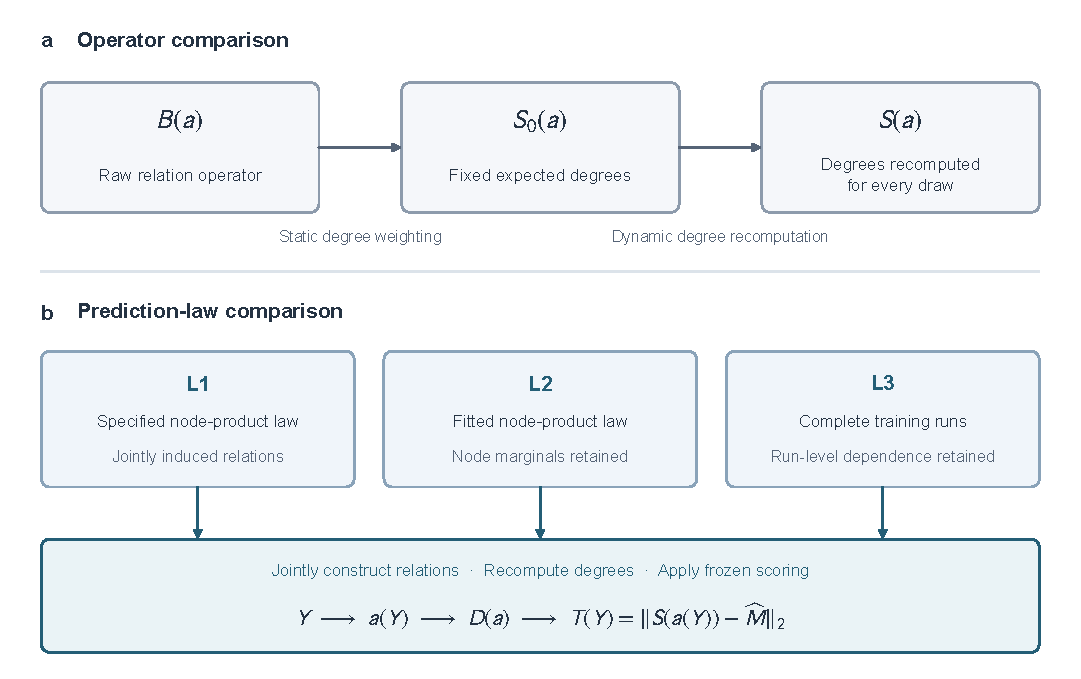
\includegraphics[width=\textwidth]{figures/operator_law_map.pdf}
\caption{The operator comparison and the prediction-law comparison are
distinct axes. (a) $B\to S_0\to S$ separates static weighting from dynamic
normalization. (b) L1--L3 specify which joint prediction mechanism generates
the relation draws used by the same normalized score.}
\label{fig:calibration-map}
\end{figure}

\section{Normalized Node Influence}\label{sec:normalized-influence}

Normalization changes the conditional response, but it does not remove
the conditional-expectation decomposition. Let
$X^S=S(Y)-\mathbb E S(Y)$ under L1 and define
\begin{equation}\label{eq:normalized-influence}
F_u^S(z)=\mathbb E[S(Y)\mid Y_u=z]-\mathbb E S(Y),\qquad
R^S=X^S-\sum_uF_u^S(Y_u).
\end{equation}

\begin{proposition}[Normalized conditional influence]\label{prop:norm-influence}
For independent node coordinates and finite second moments,
$\mathbb E[R^S\mid Y_u]=0$ for every $u$, and
\begin{equation}\label{eq:norm-energy}
\mathbb E\|X^S\|_F^2
=\sum_u\mathbb E\|F_u^S(Y_u)\|_F^2+\mathbb E\|R^S\|_F^2.
\end{equation}
For a binary coordinate with $P_0P_1>0$, put
$\Delta_u=\mathbb E[S\mid Y_u=1]-\mathbb E[S\mid Y_u=0]$.
Then $F_u^S(1)=P_0\Delta_u$, $F_u^S(0)=-P_1\Delta_u$, and
$v_u:=\mathbb E\|F_u^S(Y_u)\|_F^2=P_0P_1\|\Delta_u\|_F^2$.
\end{proposition}
\begin{proof}
Every $F_u^S$ has mean zero. For $v\ne u$, independence gives
$\mathbb E[F_v^S(Y_v)\mid Y_u]=0$, so conditioning
\eqref{eq:normalized-influence} on $Y_u$ gives zero conditional
remainder. Distinct influences, and each influence with the remainder,
are orthogonal in the expected Frobenius inner product. Expanding the
squared norm proves \eqref{eq:norm-energy}. The two binary values follow
by subtracting $P_0\mathbb E[S\mid0]+P_1\mathbb E[S\mid1]$.
\end{proof}

The proposition is the classical first-order decomposition applied to
the normalized matrix function. It identifies structure beyond degree:
two nodes with the same incident-edge count can have different
$\Delta_u$ because the remaining class profiles reinforce or cancel.
It does not assert that first-order influence dominates the remainder.
The raw-operator separation and cancellation theorems in
Appendix~\ref{sec:raw-mechanism} make their additional structure
conditions explicit. Their exact conclusions do not transfer
automatically through dynamic normalization.

The three-operator comparison makes that transfer measurable. Static
weighting changes $B$ into $S_0$, retaining common expectations. Dynamic
degrees change $S_0$ into $S$ and can change both means and fluctuations.
We therefore report a centered-norm ratio and a separate mean shift,
rather than interpreting a common-center difference as fluctuation
alone. Local derivative channels and a general perturbation bound are
given in Appendix~\ref{app:normalized-diagnostics} as supporting analysis.

\section{Calibration under a Stated Prediction Law}\label{sec:calibration}

\subsection{Reference, calibration, and evaluation}
The input is a fixed candidate hypergraph, its prediction-to-relation
map, a specified prediction law, and a target upper-tail probability
$\alpha$. The output is a frozen center, a threshold, and the law under
which the threshold is justified. The procedure has three stages.
\begin{enumerate}
\item Use independent reference observations to estimate $\widehat M$
and freeze all choices defining the score. For L2, estimate the product
law here; for L3, an observation is a complete training run.
\item Generate $M$ independent calibration observations from the chosen
law, construct all relations jointly, recompute degrees, and obtain
$T_1,\ldots,T_M$ with the frozen score.
\item For evaluation, keep the center and threshold fixed. Neither new
scores nor evaluation labels update the calibrator.
\end{enumerate}
The edge-independent baseline replaces step 2 by independent edge-slot
sampling at the same specified or fitted marginals. This changes the
calibration law; it does not inherit the node-law guarantee.

\subsection{Rank threshold and its probability target}
Let $T_{(1)}\le\cdots\le T_{(M)}$ and define
\begin{equation}\label{eq:rank-threshold}
k=\left\lceil(M+1)(1-\alpha)\right\rceil,\qquad
q_\alpha=\begin{cases}T_{(k)},& k\le M,\\+\infty,& k>M.\end{cases}
\end{equation}
An alarm is the strict event $T_{\mathrm{new}}>q_\alpha$.

\begin{proposition}[Law-specific rank validity]\label{prop:rank}
Condition on the independent reference stage. If the calibration
scores and a new score are exchangeable under a law $\mathcal L$, then
\begin{equation}\label{eq:rank-validity}
\Pr_{\mathcal L}\{T_{\mathrm{new}}>q_\alpha\mid\mathrm{reference}\}
\le\alpha.
\end{equation}
The probability averages jointly over calibration observations and
the new observation. With ties, the strict rule is conservative.
\end{proposition}
\begin{proof}
Break ties by independent random ordering. Exchangeability makes the
new observation's rank uniform on $1,\ldots,M+1$. Strict exceedance of
the $k$th calibration score implies a rank greater than $k$, giving
probability at most $(M+1-k)/(M+1)\le\alpha$. Removing the random
tie-breaking can only remove strict exceedances. If $k>M$ the event is
empty.
\end{proof}

This is the standard rank argument \cite{vovk2012conditional}.
Within L1 it applies to node draws and their jointly induced edges.
Within a frozen fitted product law it applies to L2 draws from that law,
not automatically to real training runs. Under L3 it applies to fresh
exchangeable complete runs of the same protocol. Repeatedly resampling
a finite run pool is not itself evidence of exchangeability with a
fresh training run.

\subsection{Interpreting empirical exceedance}
The realized threshold's conditional exceedance probability need not
equal $\alpha$ or satisfy \eqref{eq:rank-validity} conditional on that
particular calibration sample. Binomial Clopper--Pearson intervals
describe evaluation variability for a frozen threshold; including
$\alpha$ in such an interval does not prove equivalence. Across batches
with different fitted centers and thresholds, pooled evaluation
indicators need not have a common success probability. We report
batch-specific intervals or their explicitly labeled endpoint envelope.

\section{Experiments}\label{sec:exp}

The main experiments ask three consecutive questions: what
normalization changes, whether the chosen law supports calibration,
and whether a fitted node product reproduces complete training runs.
Cora-CC and DBLP-CA use AllSet benchmark inputs
\cite{chien2022allset}; their candidate structures contain 2,708/41,302
nodes and 1,579/22,363 edge slots. The controlled normalization families
use 120 edges per hub and are distinct from the larger raw-operator
grids retained in Appendix~\ref{sec:raw-validation}. All numerical
comparisons use the operator in \eqref{eq:norm-operator}.

\paragraph{Numerical and statistical protocol.}
Reference, calibration, and evaluation stages use separate seed streams.
Small matrices use dense symmetric eigendecomposition. Larger matrices
use both algebraic ends of a sparse eigensolver with a fixed start,
and the implementation can return an approximation or fallback score.
The rank guarantee applies to the shared implemented score, not to a
certified exact spectral norm. For large-scale DBLP matrices, raw and
fixed-degree spectral scores are computed with iterative sparse
eigensolvers as point estimates (marked with $\dagger$ in
Table~\ref{tab:normalization}), whereas rank-calibration guarantees
apply directly to the shared implemented scoring pipeline.

\subsection{Normalization changes the dependence comparison}
Dynamic normalization attenuated the estimated centered-norm ratio on
all displayed native units, while their computed ratios remained above
one (Table~\ref{tab:normalization}). The native dynamic ratios ranged
from 1.03 to 1.26, compared with raw ratios of 2.15--3.47.
The coherent controlled family instead changed from 2.93 for $B$ to
0.24 for $S$, accompanied by a normalized mean shift of 0.532.
These outcomes separate raw amplification from normalized behavior.
They do not attribute a fluctuation difference to mean shift alone,
because the ratios use each arm's own estimated mean.

% Generated from frozen results by notes/calibration-integration/generate_tables.py
\begin{table}[htbp]
\centering\small
\setlength{\tabcolsep}{4pt}
\begin{tabular}{llrrrr}
\toprule
Structure & Profile & $R_B$ & $R_{S_0}$ & $R_S$ & $\Delta_\mu$ \\
\midrule
Coherent & aligned & 2.93 & 1.16 & 0.24 & 0.53 \\
Competition & $\gamma=.05$ & 1.01 & 1.00 & 1.00 & 0.02 \\
Competition & $\gamma=.50$ & 1.40 & 1.02 & 0.99 & 0.09 \\
Competition & $\gamma=.95$ & 2.28 & 0.85 & 0.53 & 0.44 \\
Cora & binary .05 & 3.25 & 1.39 & 1.24 & 0.08 \\
Cora & binary .15 & 2.93 & 1.41 & 1.09 & 0.18 \\
Cora & multi .05 & 3.47 & 1.24 & 1.26 & 0.08 \\
Cora & multi .15 & 3.28 & 1.29 & 1.11 & 0.17 \\
Cora & hetero & 3.23 & 1.45 & 1.05 & 0.23 \\
DBLP$^\dagger$ & binary .05 & 2.48 & 1.70 & 1.13 & 0.19 \\
DBLP$^\dagger$ & binary .15 & 2.16 & 1.42 & 1.03 & 0.29 \\
DBLP$^\dagger$ & hetero & 2.15 & 1.77 & 1.07 & 0.34 \\
\bottomrule
\end{tabular}
\caption{Computed mean centered-norm ratios A/B; $\Delta_\mu=\|\widehat{\mathbb E}_A S-\widehat{\mathbb E}_B S\|_2$. Dynamic norms use each arm's own estimated mean; raw and fixed-degree means match analytically. Center/evaluation budgets per arm are 800/600 for the controlled families and Cora, and 120/80 for DBLP. Native binary/multiclass profiles have the displayed error probability; hetero uses binary errors at .02 below the upper degree decile and .30 within it. $\dagger$ DBLP raw/fixed-control scores include numerical approximations; these are point estimates, not certified norm ratios.}
\label{tab:normalization}
\end{table}


Exact small-graph enumeration verified the normalized conditional
orthogonality and energy identity to numerical precision. On the
degree-120 controlled hubs, estimated $v_u$ was 1.099 for the coherent
profile, approximately zero at the competing flat profile, and 1.311
at the aligned competing-family endpoint. Thus equal degree did not
fix normalized influence energy. Native influence estimates used
selected high-impact and background nodes; no full-native energy
closure is claimed.

\subsection{Model-law calibration and separate-seed reanalysis}
Preserving node-induced relations sharply changed calibration under
known node laws (Table~\ref{tab:node-calibration}). At target $\alpha=5\%$,
native node-calibrated batch means ranged from 3.9\% to 5.9\%, while
independent-edge thresholds yielded 47.5\%--100\% exceedance under the
same node mechanism. These are model-law comparisons: the labels used
to define the artificial errors are known to the simulator. Heterogeneous
calibration profiles use multiclass errors; the heterogeneous normalization
profiles in Table~\ref{tab:normalization} instead use binary errors.

% Generated from frozen results by notes/calibration-integration/generate_tables.py
\begin{table}[htbp]
\centering\small
\setlength{\tabcolsep}{4pt}
\begin{tabular}{llrr}
\toprule
Structure & Profile & Node (\%) & Edge-iid (\%) \\
\midrule
Cora & binary .05 & 5.2 [3.7,7.2] & 99.5 [98.3,100.0] \\
Cora & binary .15 & 5.0 [3.6,6.7] & 97.7 [95.6,99.4] \\
Cora & hetero & 5.9 [3.0,9.3] & 47.5 [40.5,54.9] \\
Cora & multi .05 & 4.8 [3.3,6.5] & 99.7 [98.7,100.0] \\
Cora & multi .15 & 5.5 [2.9,8.3] & 99.0 [97.5,99.9] \\
DBLP & binary .05 & 4.6 [1.4,9.3] & 100.0 [98.8,100.0] \\
DBLP & binary .15 & 5.1 [1.4,10.1] & 96.8 [90.7,99.8] \\
DBLP & hetero & 3.9 [0.9,8.9] & 99.7 [97.1,100.0] \\
Coherent & aligned & 0.0 [0.0,0.2] & 9.2 [7.8,10.7] \\
\bottomrule
\end{tabular}
\caption{Known-node-law exceedance at $\alpha=5\%$. Native entries are means over three independent threshold batches; brackets give the minimum lower and maximum upper endpoint of their individual 95\% binomial intervals, not a pooled 95\% interval. Per-batch reference/calibration/evaluation budgets are 200/500/1000 on Cora and 80/150/300 on DBLP. Hetero here uses multiclass errors at .02/.30. The coherent-family row is one batch with 400/800/1600 observations.}
\label{tab:node-calibration}
\end{table}


The controlled coherent family illustrates conservative ties. Its
5\% node threshold had zero strict exceedances in 1,600 evaluations,
because a discrete upper-tail atom determined the threshold. Zero
exceedance does not establish useful detection power, even when rank
validity holds. In the fitted-law Cora pilot, the three-repeat mean
5\% exceedance was approximately 5.0\% within the fitted model and
4.9\% under the specified generating law. That observation concerns
a weak-error synthetic product law, not the training-induced L3 law.

A fresh three-batch Cora rerun produced rates of 6.9\%, 3.3\%, and
4.9\%, for a mean of 5.03\% across 3,000 evaluations
(Table~\ref{tab:cora-rerun}). The batch-specific 95\% intervals have
an endpoint envelope of 2.28\%--8.65\%. Because centers and thresholds
differ by batch, this envelope is not a pooled interval. The three-batch
mean exceedance rate was 5.03\%, consistent with the nominal 5\% target
at this resolution.

% Generated from frozen results by notes/calibration-integration/generate_tables.py
\begin{table}[htbp]
\centering\small
\setlength{\tabcolsep}{4pt}
\begin{tabular}{rrrrr}
\toprule
Batch & Exceedances & Rate (\%) & CP 95\% interval & $q_{.05}$ \\
\midrule
1 & 69/1000 & 6.9 & [5.4,8.7] & 0.790 \\
2 & 33/1000 & 3.3 & [2.3,4.6] & 0.764 \\
3 & 49/1000 & 4.9 & [3.6,6.4] & 0.782 \\
\bottomrule
\end{tabular}
\caption{Fresh Cora-CC rerun under the specified binary node-product law. Each batch uses 200/500/1000 reference/calibration/evaluation draws and a distinct deterministic seed. Intervals are batch-specific conditional Clopper--Pearson intervals; the endpoint envelope is not a pooled interval. The three-batch mean exceedance rate was 5.03\%, consistent with the nominal 5\% target at this resolution.}
\label{tab:cora-rerun}
\end{table}


\subsection{Complete training runs expose product-law mismatch}
The product of empirical node frequencies produced zero observed
exceedances in every displayed L3 setting (Table~\ref{tab:run-calibration}).
Whole-run thresholds instead produced nonzero exceedances with broad
conditional intervals. In the two fixed-training-set GCN settings,
the run-pool counts at 5\% were 1/60 on Cora and 1/40 on DBLP;
the corresponding node-product counts were zero. These observations
support using complete runs as the practical calibration baseline for
the tested mechanisms. They do not establish uniqueness or universal
superiority of this baseline.

% Generated from frozen results by notes/calibration-integration/generate_tables.py
\begin{table}[htbp]
\centering\small
\setlength{\tabcolsep}{4pt}
\begin{tabular}{lllrrr}
\toprule
Data & Mechanism & R/C/E & Run-pool (\%) & Node-fit & Edge-iid \\
\midrule
Cora & LP & 50/100/100 & 4.0 [1.1,9.9] & 0.0 & 0.0 \\
DBLP & LP & 40/80/80 & 6.2 [2.1,14.0] & 0.0 & 0.0 \\
Cora & Proto & 30/100/150 & 3.3 [1.1,7.6] & 0.0 & 9.3 \\
DBLP & Proto & 20/50/80 & 6.2 [2.1,14.0] & 0.0 & 0.0 \\
Cora & GCN-XF & 20/40/60 & 6.7 [1.8,16.2] & 0.0 & 0.0 \\
Cora & GCN-init & 20/40/60 & 1.7 [0.0,8.9] & 0.0 & 0.0 \\
DBLP & GCN-init & 15/25/40 & 2.5 [0.1,13.2] & 0.0 & 0.0 \\
\bottomrule
\end{tabular}
\caption{Whole-run evaluation at $\alpha=5\%$. R/C/E are the reference/calibration/evaluation run counts. All rates are percentages; run-pool brackets are conditional 95\% binomial intervals for the realized threshold. LP varies labeled subsets, Proto varies a half split, GCN-XF uses five-fold cross-fitting, and GCN-init holds a 20\% labeled subset fixed. Zero node-fit counts do not imply zero population probability; their upper 95\% endpoints range from 2.4\% to 8.8\%. Every 5\% threshold displayed is finite.}
\label{tab:run-calibration}
\end{table}


The random mechanisms differ deliberately. LP varies the labeled
subset; prototype prediction varies a half split; cross-fit GCN varies
fold assignments and initialization. The final two rows hold a 20\%
labeled subset fixed and vary initialization only, using 500 epochs on
Cora and 120 on DBLP. The calibration/evaluation separation is at the
run level in each case. No DBLP cross-fit GCN row is inferred from the
fixed-split experiment.

At $\alpha=10\%$, the fixed-split run-pool counts were 9/60 on Cora
and 1/40 on DBLP. Their intervals included the target but were too
wide to establish equivalence. At $\alpha=1\%$, calibration pools of
25, 40, 50, or 80 runs cannot yield a finite threshold under
\eqref{eq:rank-threshold}; zero alarms at $q=\infty$ convey no
detection ability. More simulation from a fitted node product cannot
repair missing dependence in the model being simulated.

\subsection{Cross-domain calibration on visual object hypergraphs}\label{sec:visual}
We extended the complete-run protocol to two preprocessed visual object
hypergraphs from the ED-HNN benchmark~\cite{wang2023edhnn}: NTU2012 (2,012 objects, 67
classes, 2,012 five-object hyperedges) and ModelNet40 (12,311 objects,
40 classes, 12,311 five-object hyperedges). Object features and labels
were matched to the released incidence data by identifier, excluding
auxiliary hyperedge-node rows. A two-layer fixed propagation predictor
$S_{\mathrm{all}}\mathrm{ReLU}(S_{\mathrm{all}}XW_1)W_2$ used a fixed
stratified 60/20/20 training/validation/test split. Its output generated
the monitored operator $S(Y)$. Each dataset supplied one batch of 30
reference, 99 calibration and 200 independent evaluation runs, for
658 complete training runs across the two datasets.

The fitted node-product calibration remained conservative across
these visual domains (Table~\ref{tab:visual-alarm-validation}). At
$\alpha=5\%$, it yielded zero exceedances in 200 evaluation runs on
each dataset (upper CP endpoint $1.83\%$), extending the direction
observed on Cora-CC and DBLP-CA. Independent-edge calibration instead
yielded 10/200 exceedances on NTU and 53/200 ($26.5\%$) on ModelNet.
Thus preserving edge marginals or fitted node marginals did not
reproduce the calibration behavior of the complete-run law.

% Generated from frozen visual_alarm_v1 results by notes/calibration-integration/generate_tables.py
\begin{table}[t]
\centering\small
\setlength{\tabcolsep}{3pt}
\begin{tabular}{lccccc}
\toprule
Dataset & \multicolumn{3}{c}{Clean exceedance (\%; 95\% CP interval)} & Resplit & Time (s) \\
\cmidrule(lr){2-4}
 & L3 & L2 & Edge-iid & mean (\%) & train/score \\
\midrule
NTU2012 & 14.0 [9.5,19.6] & 0.0 [0.0,1.8] & 5.0 [2.4,9.0] & 5.0 & 3.5/0.04 \\
ModelNet40 & 5.5 [2.8,9.6] & 0.0 [0.0,1.8] & 26.5 [20.5,33.2] & 5.0 & 56.2/0.26 \\
\bottomrule
\end{tabular}
\caption{Cross-domain calibration at $\alpha=5\%$. Each dataset uses
30 reference, 99 calibration and 200 independent evaluation complete
runs. L3 calibrates on complete runs, L2 on a fitted node-product law,
and Edge-iid on independently sampled edge events. Brackets are
batch-specific $95\%$ Clopper--Pearson intervals. Resplit means use
10,000 random 99/200 partitions of the same 299 scores with a frozen
reference center; they are internal sensitivity summaries, not
independent validation. Timing gives median training/spectral-scoring
seconds per complete run under the recorded six-way parallel setup.}
\label{tab:visual-alarm-validation}
\end{table}


Complete-run calibration also exposes the distinction between marginal
and conditional validity. Its frozen threshold yielded 28/200
($14.0\%$) exceedances on NTU and 11/200 ($5.5\%$) on ModelNet.
Proposition~\ref{prop:rank} averages over the calibration
sample and the next exchangeable run; it does not require each frozen
threshold's conditional exceedance probability to equal $5\%$.
Figure~\ref{fig:visual-alarm-validation} compares the observed rates
with internal split sensitivity. With the reference center frozen,
10,000 random 99/200 splits of the same 299 NTU scores gave mean
exceedance $5.0\%$, median $4.5\%$, and 97.5th percentile $11.0\%$;
the original threshold lay at the 0.4th percentile of resampled
thresholds. ModelNet also gave a split mean of $5.0\%$. This
finite-pool rank check illustrates conditional variability; repeated
use of the same runs is not an independent population-level test of
the marginal guarantee.

\begin{figure}[t]
\centering
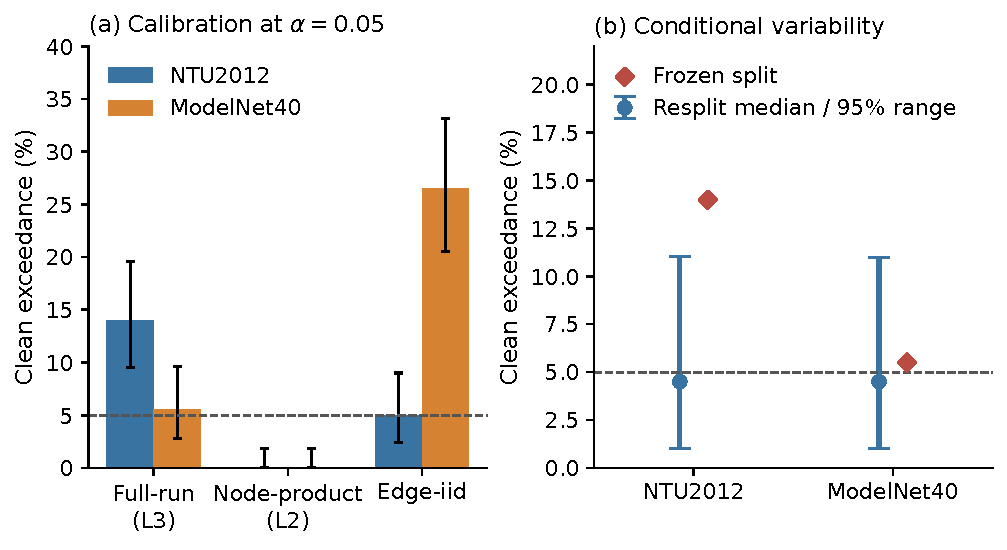
\includegraphics[width=\textwidth]{figures/visual_alarm_main.pdf}
\caption{Cross-domain calibration and frozen-threshold variability.
(a) Clean exceedance for complete-run (L3), fitted node-product (L2),
and independent-edge calibration at $\alpha=5\%$; horizontal error bars are
batch-specific $95\%$ Clopper--Pearson intervals from 200 evaluation
runs. (b) Original frozen-split rates and the median and central
$95\%$ range of 10,000 random 99/200 splits of the same 299 scores,
conditional on the frozen reference center. The split range is an
internal sensitivity summary, not a confidence interval for the
population risk. Dashed lines mark the $5\%$ target.}
\label{fig:visual-alarm-validation}
\end{figure}

A deployment requirement on the conditional risk of a frozen threshold
calls for an additional calibration criterion. Under an independently
and identically distributed run mechanism, a binomial tolerance rule
controls the probability that this conditional risk exceeds
$\alpha$, with confidence parameter $1-\delta$
\cite{vovk2012conditional}. At $M=99$ and
$\alpha=\delta=5\%$, it uses the 98th rather than the 95th ordered
score. On the same evaluation runs this gives 19/200 ($9.5\%$) on NTU
and 3/200 ($1.5\%$) on ModelNet. These realized rates remain distinct
from the rule's probability statement over calibration samples. The
tolerance comparison reuses the observed evaluation data; the
original thresholds and counts are retained. Appendix~\ref{app:visual}
gives the criterion, numerical sensitivity, and secondary
feature-perturbation comparisons.

\section{Discussion and Limitations}\label{sec:limits}

The results locate two distinct failures of a calibration shortcut.
Within a known independent-node model, treating induced edge events
as independent can produce severe over-exceedance. With real training
runs, a product of fitted node marginals can instead yield an overly
conservative threshold. The direction of failure depends on which
joint law is omitted. Consequently, preserving shared-node dependence
recovers the specified node-model construction but does not by itself
recover a training-run distribution.

Normalization explains why the raw theory is a starting point rather
than a sufficient calibration model. It can attenuate fluctuations,
shift expectations, or change the direction of a controlled comparison.
Conditional influence quantifies this change without assuming the
remainder is small. Its energy is structural information, not a proved
optimal monitoring direction. Appendix~\ref{app:normalized-diagnostics}
gives a local-response formula and perturbation bound as supporting tools.

The guarantees retain explicit boundaries. Known node laws need not
describe shared training states; fitted frequencies need not represent
repeated-run probabilities; and a fixed data set and training protocol
do not cover a new graph or a changed training process. The
Cora-CC/DBLP-CA L3 evaluation pools are small and lack a new
prospective confirmation with retained run-level prediction caches.
The visual protocol retains run-level caches for two additional
datasets under its stated single-batch 30/99/200 design. All runs in
a calibration claim must remain exchangeable under its declared
mechanism.

The visual benchmarks extend the distinction between joint laws to a
different data domain. Fitted node products remained conservative on
both, while independent-edge calibration gave substantial
exceedance on ModelNet40. The NTU frozen threshold and split-sensitivity
analysis further separate the probability target from any one
realization: marginal rank validity does not give a high-confidence
bound on the conditional risk of every deployed threshold. Binomial
tolerance calibration provides an established way to express the
latter objective under an independent-run model. More calibration
runs can reduce sampling variation, but the probability target and
assumed law must first be specified.

Numerical precision is a separate restriction. The DBLP entries in
Table~\ref{tab:normalization} are computed-score evidence; certified
spectral-norm magnitudes require an independent numerical audit. The ES
importance estimates also do not provide a usable tail certificate:
their effective-sample diagnostics were low and tested bounds were
vacuous. Stronger remainder bounds and risk-weighted propagation are
outside the present claim.

\section{Conclusion}\label{sec:conclusion}
Normalized spectral-risk calibration requires a declared joint
prediction law. Conditional influence separates the effects of
normalization from raw-operator fluctuation, while rank calibration
states validity under the corresponding exchangeability assumption.
Controlled families, citation networks and visual object hypergraphs
show different calibration consequences of omitting shared-node
relations or training-run dependence. Complete-run and split-sensitivity
comparisons further distinguish marginal validity from the conditional
behavior of a frozen threshold. These results guide the construction
and interpretation of upstream operator-deviation alarms.


\section*{Data and Code Availability}
The complete source code, frozen configurations, certificates, saved
measurements, and reproducibility instructions for both the normalized
calibration experiments and the raw-operator mechanism checks are publicly
available at\\
\url{https://github.com/pengshen1212/hypergraph-spectral-fluctuations}.
The normalized calibration materials are also provided in the accompanying
submission package.
Cora-CC and DBLP-CA inputs are available through
\href{https://github.com/jianhao2016/AllSet}{AllSet}; preprocessed
NTU2012 and ModelNet40 visual hypergraphs are obtained from the public
\href{https://github.com/Graph-COM/ED-HNN}{ED-HNN benchmark repository}~\cite{wang2023edhnn}.
The retained raw
Walmart experiments use
\href{https://www.cs.cornell.edu/~arb/data/walmart-trips/}{Austin R. Benson's dataset collection}.
Third-party inputs are not redistributed in the revision package.

\section*{CRediT Authorship Contribution Statement}
\textbf{Shen Peng:} Conceptualization, Methodology, Formal analysis,
Validation, Software, Investigation, Data curation.
\textbf{Rui Wang:} Investigation, Data curation.
\textbf{Yunchao He:} Writing -- original draft, Writing -- review and editing.

\section*{Funding}
This work received no specific funding from public, commercial, or
non-profit funding agencies.

\section*{Declaration of Competing Interest}
The authors declare that they have no competing interests.

\section*{Declaration of Generative AI and AI-Assisted Technologies
in the Manuscript Preparation Process}
ChatGPT (OpenAI) was used for literature discovery, assistance with
intermediate mathematical derivations, and language revision.
Codex (OpenAI) assisted manuscript organization, reference verification,
language revision, and preparation of the explanatory diagram's source.
The authors are responsible for checking the derivations, references,
and final manuscript and for the content of the published article.

\section*{Acknowledgements}
The authors thank Jianjia Wang for guidance during this research.

\bibliographystyle{elsarticle-num}
\bibliography{references}

\clearpage
\appendix
% Keep appendix references as letters; add the prefix only to section headings.
\renewcommand{\thesection}{\Alph{section}}
\makeatletter
\renewcommand{\@seccntformat}[1]{\ifstrequal{#1}{section}{Appendix~}{}\csname the#1\endcsname.\quad}
\makeatother
\numberwithin{table}{section}
\numberwithin{figure}{section}
\numberwithin{equation}{section}

\section{Raw-Operator Model and Mechanism}\label{sec:raw-mechanism}\label{sec:model}
The following raw-operator theory supplies the mechanism foundation. Its matched expectations and separation claims concern the unnormalized operator; the normalized analysis in Section~\ref{sec:normalized-influence} does not assume that these conclusions transfer.


\begin{figure}[htbp]
\centering
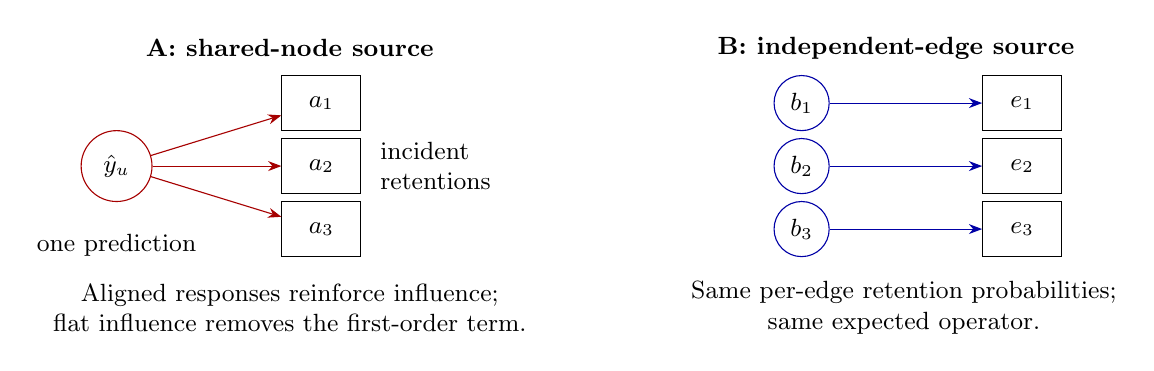
\begin{tikzpicture}[>=Stealth, font=\small,
  source/.style={circle,draw,minimum size=9mm,inner sep=1pt},
  edge/.style={draw,minimum width=10mm,minimum height=7mm,inner sep=2pt}]
\node at (3,0.7) {\textbf{A: shared-node source}};
\node[source,draw=red!65!black] (u) at (0.8,-0.8) {$\hat y_u$};
\node[align=center] at (0.8,-1.8) {one prediction};
\foreach \i/\y in {1/0,2/-0.8,3/-1.6} {
  \node[edge] (a\i) at (3.4,\y) {$a_\i$};
  \draw[->,red!65!black] (u) -- (a\i);
}
\node[align=left,text width=23mm] at (5.3,-0.8) {incident\\retentions};
\node at (10.7,0.7) {\textbf{B: independent-edge source}};
\foreach \i/\y in {1/0,2/-0.8,3/-1.6} {
  \node[source,minimum size=7mm,draw=blue!65!black] (b\i) at (9.5,\y) {$b_\i$};
  \node[edge] (e\i) at (12.3,\y) {$e_\i$};
  \draw[->,blue!65!black] (b\i) -- (e\i);
}
\node[align=center] at (3,-2.6) {Aligned responses reinforce influence;\\flat influence removes the first-order term.};
\node[align=center] at (10.8,-2.6) {Same per-edge retention probabilities;\\same expected operator.};
\end{tikzpicture}
\caption{Shared predictions couple incident relations even when each
edge has the same marginal retention probability as an independent
draw. Coherent influence measures their combined response. Norm
separation also requires the stated overlap conditions; exact
directional-variance cancellation requires every shared node to be
flat and edge pairs to share at most one node. The explanatory diagram
was drafted with Codex (OpenAI) assistance and rendered from its TikZ source.}
\label{fig:shared-source}
\end{figure}

Fix a candidate hypergraph $E$ with edge sizes $r_e\ge2$ and true
labels $y$. Node predictions $\hat y_u$ are independent with
categorical laws $P[u,c]$. These laws define the controlled
relation-construction model; Appendix~\ref{app:identification}
describes conditioning on a shared training state. Write
\[
H_e=\mathbf 1_e\mathbf 1_e^\top/r_e,\qquad
a_e=\ind{\text{all predictions on }e\text{ agree}},\qquad
p_e=\mathbb E\,a_e=\sum_c\prod_{u\in e}P[u,c].
\]
The estimated relation operator is $B(\hat a)=\sum_ea_eH_e$, an
unnormalized sum of rank-one clique contributions. With the true-label
indicator $a_e^*$, the error operator is $\Delta B_A=\sum_e(a_e-a_e^*)H_e$
and $\mathbb E\Delta B_A=\sum_e(p_e-a_e^*)H_e=:M_0$. Both arms below
are centered on this common mean, so all statements concern
\[
X_A=\sum_e(a_e-p_e)H_e,\qquad
X_B=\sum_e(b_e-p_e)H_e,\qquad b_e\sim\mathrm{Bern}(p_e)
\ \text{independently,}
\]
with $\widetilde\beta_M=\|X_M\|_2$. The conditional retention kernel
\[
g_{e,u}(z):=\mathbb E[a_e\mid \hat y_u=z]
=\prod_{v\in e\setminus\{u\}}P[v,z]
\]
is defined by re-multiplying over the remaining nodes, so zero
probability classes are handled without division. For binary laws set
$\phi_{u,e}:=g_{e,u}(1)-g_{e,u}(0)$ and, for a fixed unit vector $x$,
\[
h_e(x):=x^\top H_ex=\Bigl(\textstyle\sum_{u\in e}x_u\Bigr)^2\!/r_e\ \ge0,
\qquad
\Phi_u(x):=\sum_{e\ni u}\phi_{u,e}\,h_e(x).
\]
$\Phi_u(x)$ is node $u$'s \emph{coherent influence} at $x$: the amount
by which its prediction moves the incident weighted retention sum.

The homogeneous submodel has all
candidate edges $r$-uniform and homogeneous, i.i.d.\ binary flips
$W_u\sim\mathrm{Bernoulli}(p)$, $q_r=1-(1-p)^r-p^r$. There,
$g_{e,u}(1)=(1-p)^{r-1}$, $g_{e,u}(0)=p^{r-1}$, and
$\phi_{u,e}=\pm\bigl[(1-p)^{r-1}-p^{r-1}\bigr]$ for every member of a
homogeneous edge. The general influence theory allows heterogeneous
categorical laws.



\subsection{Node-Influence Decomposition}\label{sec:decomp}

The decomposition, its second-moment identity, and the variance lower
bound form one chain and are stated together.

\begin{theorem}[Influence decomposition and variance identity]
\label{thm:decomp}
Define $F_u(z):=\sum_{e\ni u}\bigl[g_{e,u}(z)-p_e\bigr]H_e$. Then:
\begin{enumerate}
\item[\textup{(i)}] $X_A=\sum_uF_u(\hat y_u)+R$ with $\mathbb
E[R\mid\hat y_u]=0$ for every $u$; moreover $\mathbb EF_u(\hat y_u)=0$,
the components are entrywise orthogonal
($\mathbb E[F_u(\hat y_u)F_v(\hat y_v)]=0$ and $\mathbb E[F_u(\hat
y_u)R]=0$ as matrices for $u\ne v$), and
\[
\mathbb E[X_A^2]=\sum_u\mathbb E\bigl[F_u(\hat y_u)^2\bigr]+\mathbb E[R^2],
\qquad
\mathbb E[X_B^2]=\sum_ep_e(1-p_e)H_e .
\]
\item[\textup{(ii)}] For every fixed unit $x$,
\[
\operatorname{Var}(x^\top X_Ax)=V_1(x)+\operatorname{Var}(x^\top Rx)
\ \ge\ V_1(x),\qquad
V_1(x)=\sum_u\operatorname{Var}_{Z\sim P[u,\cdot]}
\Bigl[\sum_{e\ni u}g_{e,u}(Z)h_e(x)\Bigr],
\]
and in the binary case $V_1(x)=\sum_uP[u,1]P[u,0]\,\Phi_u(x)^2$ with
the single-term bound
$V_1(x)\ge m_u(1-m_u)\Phi_u(x)^2$, $m_u=\min_cP[u,c]$.
\end{enumerate}
\end{theorem}

\begin{proposition}[Covariance form of the A/B gap]\label{prop:cov}
$\mathbb E[X_A^2]-\mathbb E[X_B^2]
=\sum_{e\ne f}\operatorname{Cov}(a_e,a_f)\,H_eH_f$, a symmetric
operator identity; $\operatorname{Cov}(a_e,a_f)=0$ whenever
$e\cap f=\varnothing$, and for a pair sharing exactly one node $u$,
$\operatorname{Cov}(a_e,a_f)
=\mathbb E_{Z\sim P[u,\cdot]}\bigl[g_{e,u}(Z)g_{f,u}(Z)\bigr]-p_ep_f$.
For every fixed unit $x$,
\[
\operatorname{Var}(x^\top X_Ax)-\operatorname{Var}(x^\top X_Bx)
=2\!\!\sum_{e<f,\,e\cap f\ne\varnothing}\!\!
\operatorname{Cov}(a_e,a_f)\,h_eh_f .
\]
\end{proposition}

The proofs (Appendix~\ref{app:proofs-influence}) use
$F_u(\hat y_u)=\mathbb E[X_A\mid\hat y_u]$ per
Theorem~\ref{thm:decomp},
and orthogonality follows from independence and zero means. No
structure assumption is made on $E$---sizes, overlaps, and label
compositions are arbitrary. The classical star variance amplification
is the special case $x=\mathbf e_v$ at a disjoint-leaf
star: $\Phi_v=d\bigl[(1-p)^{r-1}-p^{r-1}\bigr]/r$ gives
$\operatorname{Var}_A/\operatorname{Var}_B=1+(d-1)\kappa$ with
$\kappa=p(1-p)\bigl[(1-p)^{r-1}-p^{r-1}\bigr]^2/\bigl(q_r(1-q_r)\bigr)$;
e.g.\ $(r,p,d)=(3,0.05,20)$ gives $6.98$.

\begin{lemma}[Deterministic single-node deviation]\label{lem:dev}
In the binary case $x^\top F_u(\hat y_u)x=\psi_u$ takes exactly two
values, $\psi_u(1)=P[u,0]\,\Phi_u(x)$ and
$\psi_u(0)=-P[u,1]\,\Phi_u(x)$; hence
$|\psi_u|\ge m_u|\Phi_u(x)|$ surely.
\end{lemma}

\subsection{Influence Separation and Its Boundary}\label{sec:theory}

\subsubsection{Certified separation under conditioned influence}

The norm-level statement needs one structural quantity beyond
$\Phi_u$. For a fixed direction $x$ let
$L_u(x):=\sum_{e\ni u}h_e(x)$ (only edges containing the witness node
contribute when $x$ is supported on it).

\begin{theorem}[Influence separation, conditioned]\label{thm:sep}
Binary laws. Let $B_1,\dots,B_t$ be pairwise node-disjoint blocks, each
containing a hub $u_i$ with amplifying value $z_i$
($m_i=P[u_i,z_i]\le\tfrac12$), and assume \emph{no edge contains two
hubs}. Fix witnesses $x_i=\mathbf e_{u_i}$ and
assume, for every $i$:
(i) \emph{coherent influence}: with
$\Phi_i:=\sum_{e\ni u_i}\phi_{u_i,e}h_e(x_i)$ (all edges containing
$u_i$ contribute, whatever block or environment they belong to),
$|\Phi_i|\ge B$;
(ii) \emph{incoherent rest}:
$V^-=\max_i\sum_{u\ne u_i}P[u,1]P[u,0]\Phi_u(x_i)^2$ and
$\phi^-_{\max}=\max_{i,u\ne u_i}|\Phi_u(x_i)|$;
(iii) \emph{bounded co-occurrence}:
$\Lambda^2=\max_i\sum_{u\ne u_i}L_u(x_i)^2$. Then
\[
\Pr\Bigl\{\widetilde\beta_A\ \ge\ L_A^{\mathrm{inf}}\Bigr\}
\ \ge\ 1-\prod_i(1-m_i)-\eta-\eta_2 ,
\]
with
\[
L_A^{\mathrm{inf}}=\min_i(1-m_i)\,B
-\sqrt{2V^-\log(2/\eta)}-\tfrac{\phi^-_{\max}}3\log(2/\eta)
-\sqrt{2\Lambda^2\log(2/\eta_2)} .
\]
The B arm satisfies, with probability $\ge1-\delta_B$,
$\widetilde\beta_B\le U_B=\sqrt{2v_BL_n}+2L_n/3$ with
$v_B=\bigl\|\sum_ep_e(1-p_e)H_e\bigr\|_2$, $L_n=\log(2n/\delta_B)$
(the conservative Bernstein form; the tight ${+}L_n/3$ inversion also
holds);
if the deterministic condition
$L_A^{\mathrm{inf}}>U_B$
holds, then
$\Pr\{\widetilde\beta_A>\widetilde\beta_B\}\ge
1-\prod_i(1-m_i)-\eta-\eta_2-\delta_B$.
\end{theorem}

Edges may have mixed labels, arbitrary sizes, and shared co-members;
their witness co-occurrence mass enters $\Lambda^2$. At the coordinate
witness $x_i$, only edges containing $u_i$ contribute. The one-hub-per-edge
condition keeps conditioned means unchanged by other hubs. All witnesses
are fixed before sampling.
For homogeneous stars the leading constant is
$(1-p)d[(1-p)^{r-1}-p^{r-1}]/r$; cyclic overlap enters through
$\Lambda^2$. Their verification grids are in
Appendix~\ref{app:protocol}. The complementary budget certificate
for a star core with an overlapping environment is in
Appendix~\ref{app:mixed}.

\begin{corollary}[Scale separation]\label{cor:scale}
Binary laws, arbitrary overlap. If $|\Phi_{u^\ast}(x)|\ge B$ at a unit
$x$, then with $m=\min_cP[u^\ast,c]$, $\theta\in(0,1)$, and
$Z_{\max}:=\sum_eh_e(x)\ge|x^\top X_Ax|$,
\[
\Pr\Bigl\{|x^\top X_Ax|\ \ge\ \sqrt{\theta\,m(1-m)}\,B\Bigr\}
\ \ge\ (1-\theta)^2\,\frac{m(1-m)B^2}{Z_{\max}^2},
\]
by Paley--Zygmund applied to Theorem~\ref{thm:decomp}(ii) (proof in
Appendix~\ref{app:proofs-influence}); when the influence is coherent
($Z_{\max}=O(B)$) this is a constant-probability, degree-linear bound
on arbitrary overlapping structures, against
$\widetilde\beta_B=O(\sqrt{v_B\log n})$ with high probability.
\end{corollary}

\subsubsection{Cancellation boundary}\label{sec:cancel}

\begin{theorem}[Flat profiles and exact cancellation]\label{thm:cancel}
Binary laws. (i) $\phi_{u,e}=0$ iff $u$'s prediction does not change
the conditional retention of $e$; a flat edge drops out of $\Phi_u$
for every $x$, and if all of $u$'s edges are flat then $u$ contributes
nothing to $V_1(x)$ for any $x$. (ii) For a size-$3$ edge, if the two
members
$w,w'$ of $e\setminus\{u\}$ satisfy $P[w,1]=1-P[w',1]$ (a competing
pair), then $\phi_{u,e}=0$: on a triple, one competing pair zeroes
the third member's influence. (iii) If $r_e\ge3$, all members of $e$
are flat, and every member has $P[u,1]P[u,0]>0$, then all members'
laws are uniform on the two classes. (iv) If distinct edges share at
most one node and every shared node is flat on both incident edges,
then $\operatorname{Cov}(a_e,a_f)=0$ for all $e\ne f$, hence
$\operatorname{Var}(x^\top X_Ax)=\operatorname{Var}(x^\top X_Bx)$
\emph{for every} $x$: second-order cancellation is exact.
\end{theorem}

The homogeneous-star case $p=\tfrac12$ is a symmetric instance
of flatness. A one-parameter knob makes the transition explicit: for edges
$\{u,w,\ell\}$ with $P[w,1]=\beta$ and $P[\ell,1]=\gamma$,
\[
\phi_{u,e}=\beta+\gamma-1 ,
\]
so sweeping $\gamma$ from alignment ($\beta=\gamma$) to competition
($\gamma=1-\beta$) drives the hub's influence linearly to the exact
cancellation endpoint of part (iv). Section~\ref{sec:families} sweeps
this knob.

\paragraph{Higher-order dependence and norm-level separation.}
The cancellation theorem identifies directional second moments.
Spectral-norm distributions also depend on higher-order terms in $R$.
For edge pairs sharing multiple nodes, these terms can retain pair
covariance despite flat single-node profiles. Norm separation is
certified when coherent drift exceeds the remainder and co-occurrence
penalties.

\subsubsection{Conditional influence and tail-risk certification}
\label{sec:risk}

The same conditioning idea permits a native-structure risk judgment
without the overlap restrictions of Theorem~\ref{thm:sep}. Fix a
small node group $U$ from structure alone and $\tau\ge0$. For each positive-probability
state $z$, let $\pi_z=\Pr(\hat y_U=z)$ and
$M_U(z)=\mathbb E[X_A\mid\hat y_U=z]$. A nonzero direction $q_z$
is chosen from this conditional mean before evaluation; it may depend
on $z$, since the states are disjoint. Write
\[
s_z=q_z^\top q_z,\qquad
m_z=q_z^\top M_U(z)q_z,\qquad
v_z=\operatorname{Var}(q_z^\top X_Aq_z\mid z),\qquad
D_z=|m_z|-\tau s_z.
\]
Rayleigh's inequality and one-sided Cantelli give
\begin{equation}\label{eq:risk-certificate}
\Pr(\|X_A\|_2>\tau)\ \ge\ L_U(\tau)
:=\sum_z\pi_z\ell_z(\tau),\qquad
\ell_z(\tau)=
\begin{cases}
D_z^2/(v_z+D_z^2),&D_z>0,\\
0,&D_z\le0.
\end{cases}
\end{equation}
The bound uses exact conditional covariances, including overlaps
outside $U$. Appendix~\ref{app:risk} gives the calculation and calibration
guarantee. If $\tau_B$ controls B's tail at level $\alpha$ and
$L_U(\tau_B)>\alpha$, dependence is certified to invalidate that
threshold for A. When $L_U(\tau_B)\le\alpha$, the test is
inconclusive. Calibrating a replacement threshold requires a tail
upper bound or quantile analysis.


\section{Raw-Operator Validation and Predictor Comparisons}\label{sec:raw-validation}
These retained measurements concern the raw relation operator and the original per-edge calibration protocol. They are distinct from the normalized calibration experiments in Section~\ref{sec:exp}. The Walmart inputs use the categorical benchmark associated with \cite{amburg2020categorical}. All original result tables are retained below.

\subsection{Controlled structure families}\label{sec:families}

The controlled families separate the role of influence from topology
(Figure~\ref{fig:shared-source}). Aligned responses amplify fluctuation
on non-star structures; changing only the probability profile can
remove that amplification on a fixed star. Both registered families
use $256$ formal draws per point. Family A
(\emph{amplification}): $t=60$ node-disjoint blocks, each with one weak
hub ($P[u_i,1]=0.05$) and $d$ edges $\{u_i,w_j,\text{leaf}\}$ whose
co-members are strongly class-1 ($P=0.95$), with $w_j$ drawn uniformly
from a per-block pool of $d/5$; $\Lambda^2$ is computed from realized
co-occurrences. Every edge
at $u_i$ has $\phi_{u_i,e}=0.90$, so $\Phi_i=0.9\,d/3$ while all other
nodes are exactly flat ($V^-=0$). Edges overlap through the pooled
$w_j$'s, and the blocks combine heterogeneous probability profiles.
Table~\ref{tab:familyA} reports the grid. The mean centered A norm
grows linearly in $d$ (fitted slope $0.276$ on $d\in\{150,\dots,300\}$,
within $8\%$ of the theoretical $0.9/3$) while B grows more slowly;
separation frequency is $93.8$--$100\%$, above the registered
allowance $1-0.95^{60}-\eta-\eta_2-\delta_B=0.924$ throughout. With
two-sided constants and realized $\Lambda^2\in[47.6,250.0]$, the
certificate activates at $d\ge250$ (at $d=200$: $L_A=14.4$ vs
$U_B=19.7$). Disjoint-star and cyclic checks support the same
mechanism (Appendix~\ref{app:protocol}).

\begin{table}[htbp]
\centering\small
\begin{tabular}{rrrrrrr}
\toprule
$d$ & $\Phi$ & $L_A$ & $U_B$ & $\overline{\widetilde\beta}_A$ [CI] &
$\overline{\widetilde\beta}_B$ & sep.\\
\midrule
50 & 15 & $-8.2$ & 13.7 & 16.3 $[15.8,16.8]$ & 2.36 & 93.8\%\\
100 & 30 & $-1.7$ & 16.2 & 30.9 $[30.1,31.5]$ & 2.90 & 96.1\%\\
150 & 45 & 6.0 & 18.1 & 43.9 $[42.5,45.1]$ & 3.33 & 94.1\%\\
200 & 60 & 14.4 & 19.7 & 57.4 $[55.4,59.3]$ & 3.68 & 94.5\%\\
250 & 75 & 23.75 & 21.0 & 72.5 $[70.8,74.1]$ & 4.05 & 98.0\%\\
300 & 90 & 34.0 & 22.3 & 85.4 $[83.0,87.6]$ & 4.28 & 100\%\\
\bottomrule
\end{tabular}
\caption{Family A (non-star amplification, $t{=}60$, pool $d/5$ with
random reuse, $256$ draws per point). $\Phi=0.9d/3$ is the hub's
coherent influence; $L_A$ uses two-sided constants and the realized
co-occurrence $\Lambda^2$.
Certification is nonempty from $d=250$; empirical separation exceeds
the registered allowance $0.924$ everywhere.}
\label{tab:familyA}
\end{table}

Family B (\emph{competition sweep}) fixes one hub with $d=300$ edges
$\{u,w_j,\ell_j\}$, all co-members fresh. Its \emph{topology is a
star}. Only the probability profile changes: $P[u,1]=0.05$,
$P[w_j,1]=0.95$, and $P[\ell_j,1]=\gamma$, giving
$\phi_{u,e}=\gamma-0.05$. In Table~\ref{tab:familyB}, influence
falls linearly to zero and the mean centered-norm ratio falls
from $3.36$ to $0.995$. At $\gamma=0.05$, the empirical directional
variance ratio is $0.96$ with paired-bootstrap interval $[0.76,1.20]$,
covering the exact prediction $1$. Edge pairs share only the flat
hub, so Theorem~\ref{thm:cancel}(iv) gives equality in every
direction. The empirical separation frequency is $55.5\%$ at this
endpoint. Thus fixed star topology admits both amplification and
cancellation, while certification also depends on overlap structure.

\begin{table}[htbp]
\centering\small
\begin{tabular}{rrrrrr}
\toprule
$\gamma$ & $\Phi_u$ & $\overline{\widetilde\beta}_A$ &
$\overline{\widetilde\beta}_B$ & ratio & sep.\\
\midrule
0.95 & 90.0 & 8.02 & 2.39 & 3.36 & 100\%\\
0.75 & 70.0 & 6.38 & 2.47 & 2.59 & 89.8\%\\
0.55 & 50.0 & 5.03 & 2.36 & 2.13 & 79.7\%\\
0.35 & 30.0 & 3.88 & 2.52 & 1.54 & 48.8\%\\
0.15 & 10.0 & 2.76 & 2.41 & 1.14 & 42.6\%\\
0.05 & $0.00$ & 2.39 & 2.40 & 1.00 & 55.5\%\\
\bottomrule
\end{tabular}
\caption{Family B competition sweep on a star topology ($d{=}300$,
$256$ draws per point). At $\gamma=0.05$ the hub is exactly flat
($\phi_u=0$); the directional variance ratio is $0.96$ with CI
$[0.76,1.20]$ covering the predicted equality.}
\label{tab:familyB}
\end{table}

\subsection{Native applicability}\label{sec:native}

On unmodified Cora-CC and DBLP-CA, conditional influence certifies
excess alarm risk where the original concentration certificate is
empty. Independent-edge thresholds frequently flag node-driven
errors on the same fixed structure, although edge marginals and the
expected operator are matched. Thus the alarm difference concerns
the error law, rather than an underlying structural change.
The frozen error laws are majority-versus-rest binary flips
and symmetric multiclass errors: $P[u,y_u]=1-\varepsilon$, with
remaining mass $\varepsilon/(C-1)$ per other class,
$\varepsilon\in\{0.05,0.15\}$. In the binary case $y_u$ is the
binarized label. Groups consist of the maximum-degree node and its
largest weighted co-edge partner; state-specific directions follow
the largest absolute eigenvalue of $M_U(z)$ on its nonzero support.
Group-selection ties use node IDs; all positive-probability states
are retained. Exact rational moments certify the saved directions
even when eigenvectors are approximate. Groups, directions, and
moments are fixed before fresh calibration; each threshold-dependent
certificate precedes validation.

Each cell uses 2,000 fresh B calibration draws, nominal tail $5\%$,
and joint calibration confidence at least $99\%$ across eight cells.
Two independent 1,000-draw validation batches per arm give the
alarm-rate envelopes in Table~\ref{tab:native-risk}. Node-driven
alarms occur in $93.9$--$100\%$ of validation draws, against a nominal
$5\%$ independent-edge tail. All eight exact
bounds exceed $5\%$; all eight Bonferroni-adjusted A confidence lower
endpoints exceed $92\%$. Calibration confidence and familywise $95\%$
validation intervals are separate guarantees. The alarm-rate envelopes
include all 49 ambiguous norm intervals. B's $5.1\%$ endpoint is a
finite-sample validation envelope; the calibration guarantee concerns
the population tail.

\begin{table}[htbp]
\centering\small
\begin{tabular}{llrrrr}
\toprule
Graph & Error law & $\varepsilon$ & $L_U(\tau_B)$ & A alarms (\%) & B alarms (\%)\\
\midrule
Cora & Binary & 0.05 & 0.0968 & $[95.85,96.00]$ & $[4.75,4.75]$\\
Cora & Binary & 0.15 & 0.1485 & $[97.90,98.80]$ & $[3.10,3.15]$\\
Cora & Multiclass & 0.05 & 0.0969 & $[93.90,94.05]$ & $[3.95,3.95]$\\
Cora & Multiclass & 0.15 & 0.1513 & $[98.10,99.00]$ & $[3.80,3.80]$\\
DBLP & Binary & 0.05 & 0.0950 & $[100,100]$ & $[3.65,3.65]$\\
DBLP & Binary & 0.15 & 0.2550 & $[100,100]$ & $[4.15,4.20]$\\
DBLP & Multiclass & 0.05 & 0.0970 & $[100,100]$ & $[5.00,5.10]$\\
DBLP & Multiclass & 0.15 & 0.2730 & $[100,100]$ & $[3.65,3.80]$\\
\bottomrule
\end{tabular}
\caption{Native tail-risk confirmation, 48,000 fresh draws in total.
$L_U$ reports a rounded exact-model probability lower bound.
Alarm-rate envelopes pool 2,000 validation draws per arm and span the
counts allowed by ambiguous norm intervals.}
\label{tab:native-risk}
\end{table}

Earlier variance diagnostics remain in Appendix~\ref{app:risk}.

\subsection{Real predictors and per-edge calibration}
\label{sec:pipeline}

Empirical amplification also appears with trained predictors:
the node-driven arm has larger mean centered norms in every displayed
setting (Table~\ref{tab:real-main}). Real predictions vary with
training partitions or seed labels on fixed
feature matrices and hypergraphs. An independent calibration group
estimates $\hat q_e$, and an evaluation group is compared with B draws
at these rates; both arms are centered on $\hat M=\sum_es_e\hat q_eH_e$
($s_e$ the per-edge error sign). We report the ratio of mean centered
norms. The retained
settings span citation (Cora-CC), co-authorship (DBLP-CA), and
co-purchase (Walmart-trips, LP only---no node features) structures:
all displayed bootstrap lower bounds exceed one. The predictor families provide varied
sources of relation-construction errors. Calibration sensitivity and three
disjoint-seed batches are in Appendix~\ref{app:protocol}; all $24$
batch intervals remain above one (smallest lower endpoint $1.016$).

A node-marginal resampling control checks whether shared-node
construction can reproduce the observed amplification. Drawing each node's prediction
independently from its cross-fit empirical distribution reproduces
the real arm's centered norm ($3.80$ vs $3.87$ on Cora, ratio $0.98$
$[0.86,1.12]$; $2.79$ vs $2.83$ on DBLP, $0.99$ $[0.94,1.03]$), with
both arms exceeding the independent-edge arm ($\approx1.7$). On Cora,
variance along the top eigenvector of $B(a^*)$ decomposes into
$0.134$ within-edge, $0.320$ overlapping-pair, and $0.0003$
disjoint-pair contributions. The resampling and variance decomposition
are consistent with the shared-node amplification mechanism.

\begin{table}[htbp]
\centering\small
\begin{tabular}{llrrc}
\toprule
Dataset & Predictor & Accuracy & Centered A/B & 95\% interval\\
\midrule
Cora & Prototype & 0.69 & 2.359 & $[2.022,\;3.203]$ \\
DBLP & Prototype & 0.76 & 1.960 & $[1.715,\;2.523]$ \\
Cora & GCN & $0.67$ & $2.16$ & $[1.68,\;2.90]$\\
Cora & LP & $0.57$ & $2.11$ & $[1.57,\;3.17]$\\
DBLP & LP & $0.85$ & $2.08$ & $[1.67,\;2.48]$\\
Walmart & LP & $0.64$ & $4.00$ & $[2.91,\;7.51]$\\
\bottomrule
\end{tabular}
\caption{Centered A/B under per-edge calibration ($20$ calibration and
$20$ evaluation runs per cell; prototype rows from the saved
$1000$-replicate bootstrap at $N_{\mathrm{cal}}=20$, GCN/LP rows
retained from the source runs). Pointwise intervals on fixed
structures.}
\label{tab:real-main}
\end{table}

\paragraph{Secondary spectral readout.}
A fixed-$k$ projector-distance comparison to the common expected
operator separates on Cora but not DBLP
(Appendix~\ref{sec:subspace}). DBLP's positive but small gap at
$p=0.15$ permits a unique reference subspace that may be
perturbation-sensitive. With $k$ fixed, the subspace readout separates
the arms on Cora and remains unresolved on DBLP.


\clearpage
\section{Proofs of the Influence Theorems}\label{app:proofs-influence}

\begin{proof}[Proof of Theorem~\ref{thm:decomp}]
Fix $u$ and $z$. Given $\hat y_u=z$, the events
$\{a_e=1\}$ for $e\ni u$ depend on the other members through
``all equal $z$'', of probability $\prod_{v\in e\setminus\{u\}}P[v,z]$;
edges without $u$ have unchanged conditional mean. Hence
$\mathbb E[X_A\mid\hat y_u=z]=F_u(z)$, i.e.\ $F_u(\hat y_u)
=\mathbb E[X_A\mid\hat y_u]$ pathwise. Then for $R=X_A-\sum_vF_v(\hat y_v)$
and every $u$,
\[
\mathbb E[R\mid\hat y_u]
=\mathbb E[X_A\mid\hat y_u]-F_u(\hat y_u)
-\sum_{v\ne u}\mathbb E\bigl[F_v(\hat y_v)\mid\hat y_u\bigr]=0,
\]
since $\hat y_v$ is independent of $\hat y_u$ and
$\mathbb EF_v(\hat y_v)=\mathbb E\,\mathbb E[X_A\mid\hat y_v]=0$.
Orthogonality holds entrywise, which is what the matrix identity
needs: for $u\ne v$ and any entries $(i,k),(k,j)$,
$\mathbb E[(F_u)_{ik}(F_v)_{kj}]
=\mathbb E[(F_u)_{ik}]\,\mathbb E[(F_v)_{kj}]=0$ by independence
(and likewise $\mathbb E[(F_u)_{ik}R_{kj}]
=\mathbb E[(F_u)_{ik}\,\mathbb E[R_{kj}\mid\hat y_u]]=0$), so
$\mathbb E[F_uF_v]=0$ and $\mathbb E[F_uR]=0$ as matrices; in
particular the Frobenius inner products vanish.
The matrix identity follows by expanding
$\mathbb E[X_A^2]=\mathbb E[(\sum_uF_u+R)^2]$ and collecting the
zero cross terms; for $X_B$, the summands $(b_e-p_e)H_e$ are
independent, centered, and idempotent-scaled ($H_e^2=H_e$).
\end{proof}

\begin{proof}[Proof of Proposition~\ref{prop:cov}]
Expand $\mathbb E[X_A^2]$ as
\[
\sum_{e,f}\mathbb E[(a_e-p_e)(a_f-p_f)]H_eH_f.
\]
The diagonal is $\sum_ep_e(1-p_e)H_e=\mathbb E[X_B^2]$, and
$e\cap f=\varnothing$ makes $a_e,a_f$ independent (functions of
disjoint node sets). For $e\cap f=\{u\}$, conditionally on $\hat y_u$
the two events depend on disjoint node sets, so
$\mathbb E[a_ea_f\mid\hat y_u]=g_{e,u}(\hat y_u)g_{f,u}(\hat y_u)$.
The quadratic-form identity is the same expansion evaluated at $x$;
$(H_eH_f)^\top=H_fH_e$ keeps the sum symmetric.
\end{proof}

\begin{proof}[Proof of Theorem~\ref{thm:decomp}(ii) and
Lemma~\ref{lem:dev}]
Write $x^\top X_Ax=\sum_u\psi_u+\rho$ with
$\psi_u=x^\top F_u(\hat y_u)x$ and $\rho=x^\top Rx$. The pairs
$(\psi_u,\psi_v)$ ($u\ne v$) and $(\psi_u,\rho)$ are uncorrelated by
the orthogonality above, so the variance splits as claimed. In the
binary case $\psi_u(z)=\sum_{e\ni u}(g_{e,u}(z)-p_e)h_e$ with
$p_e=P[u,1]g_{e,u}(1)+P[u,0]g_{e,u}(0)$, giving
$\psi_u(1)=P[u,0]\Phi_u(x)$, $\psi_u(0)=-P[u,1]\Phi_u(x)$, and
$\operatorname{Var}(\psi_u)=P[u,1]P[u,0]\Phi_u(x)^2$.
\end{proof}

\begin{proof}[Proof of Theorem~\ref{thm:sep}]
Let $E_i'=\{\hat y_{u_i}=z_i,\ \hat y_{u_j}\ne z_j\ \forall j<i\}$ be
the \emph{first realized} block events; they are disjoint with
$\bigcup_iE_i'=\{\exists i:\hat y_{u_i}=z_i\}$, of probability
$1-\prod_i(1-m_i)$. Fix $i$ and work conditionally on $E_i'$; under
this conditioning $\hat y_{u_i}=z_i$ and every earlier hub is pinned
at its non-amplifying value, while every non-hub node's prediction
keeps its unconditional law. By the no-shared-hub hypothesis, no edge
at the witness $x_i$ contains any hub other than $u_i$ (edges without
$u_i$ have $h_e(x_i)=0$), so pinned earlier hubs enter no term below.
Decompose
\[
x_i^\top X_Ax_i
=\underbrace{\sum_{e\ni u_i}\bigl(g_{e,u_i}(z_i)-p_e\bigr)h_e}_{=:D}
+\underbrace{\sum_{u\ne u_i}\psi_u}_{=:S}
+\underbrace{x_i^\top Rx}_{=:\rho},
\]
which is exact because $x_i^\top X_Ax_i=\psi_{u_i}+\sum_{u\ne
u_i}\psi_u+\rho$ by Theorem~\ref{thm:decomp} and
$\psi_{u_i}=D$ on $E_i'$.
\emph{Drift.} From $p_e=m_ig_{e,u_i}(z_i)+(1-m_i)g_{e,u_i}(\bar z_i)$,
\[
g_{e,u_i}(z_i)-p_e=(1-m_i)\bigl(g_{e,u_i}(z_i)-g_{e,u_i}(\bar z_i)
\bigr)=\pm(1-m_i)\phi_{u_i,e},
\]
so $D=\pm(1-m_i)\Phi_i$ and $|D|\ge(1-m_i)B\ge\min_j(1-m_j)B$.
\emph{First-order rest.} Every other hub has
$\psi_{u_j}(x_i)\equiv0$ (no edge contains both $u_i$ and $u_j$), so
$S$ runs over non-hub nodes only: their $\psi_u$ are functions of the
independent $\hat y_u$, whose laws the conditioning does not touch,
and each is centered (Theorem~\ref{thm:decomp}), bounded
$|\psi_u|\le|\Phi_u(x_i)|\le\phi^-_{\max}$ by
Lemma~\ref{lem:dev}, with variance sum $\le V^-$; a one-sided
Bernstein bound applied to $S$ and to $-S$, each at level $\eta/2$,
gives
$\Pr\{|S|>\sqrt{2V^-\log(2/\eta)}+\tfrac{\phi^-_{\max}}3
\log(2/\eta)\mid E_i'\}\le\eta$.
\emph{Remainder.} Since
$x_i^\top X_Ax_i=\sum_{e\ni u_i}(a_e-p_e)h_e$, we can write
$\rho=W-S$ with
$W=\sum_{e\ni u_i}\bigl(a_e-g_{e,u_i}(z_i)\bigr)h_e$, which depends
only on the non-hub members of $u_i$'s edges. Hence
$\mathbb E[\rho\mid E_i']
=\mathbb E[W\mid\hat y_{u_i}=z_i]-\mathbb E[S\mid E_i']=0-0$.
Changing $\hat y_u$ for a non-hub $u$ changes
$x_i^\top X_Ax_i$ by at most $\sum_{e\ni u,u_i}h_e\le L_u(x_i)$ and
changes $\psi_u$ by exactly $|\Phi_u(x_i)|\le L_u(x_i)$
(Lemma~\ref{lem:dev}); changing a hub $\hat y_{u_j}$ ($j\ne i$)
changes neither $x_i^\top X_Ax_i$ nor any term above, so its
Lipschitz constant is $0$. McDiarmid with constants $2L_u(x_i)$ gives
$\Pr\{|\rho|>\sqrt{2\Lambda^2\log(2/\eta_2)}\mid E_i'\}\le\eta_2$.
Combining by the reverse triangle inequality
$|D+S+\rho|\ge|D|-|S|-|\rho|$: on $E_i'$, with conditional
probability $\ge1-\eta-\eta_2$,
\[
\widetilde\beta_A\ \ge\ |x_i^\top X_Ax_i|\ \ge\ (1-m_i)B
-\sqrt{2V^-\log(2/\eta)}-\tfrac{\phi^-_{\max}}3\log(2/\eta)
-\sqrt{2\Lambda^2\log(2/\eta_2)} .
\]
The witness family $\{x_i\}$ is fixed before sampling; only the
realized first block is used, through the bound above. Summing the
failure probabilities over the disjoint $E_i'$,
$\sum_i\Pr(E_i')(\eta+\eta_2)\le\eta+\eta_2$, and adding the B event
(matrix Bernstein, independent summands
$(b_e-p_e)H_e$ with $\norm{\cdot}_2\le1$ a.s.) gives the claim.
\end{proof}

\begin{proof}[Proof of Corollary~\ref{cor:scale}]
$Z=x^\top X_Ax$ is centered with
$\operatorname{Var}(Z)\ge V_1(x)\ge m(1-m)B^2$
(Theorem~\ref{thm:decomp}(ii)) and $|Z|\le Z_{\max}$ surely. By
Paley--Zygmund applied to $Z^2$,
$\Pr\{Z^2\ge\theta\mathbb E Z^2\}\ge(1-\theta)^2(\mathbb EZ^2)^2/
\mathbb EZ^4$, and since $\mathbb E Z^4\le Z_{\max}^2\,\mathbb E Z^2$,
the ratio is at least $(1-\theta)^2\,\mathbb EZ^2/Z_{\max}^2\ge
(1-\theta)^2\,m(1-m)B^2/Z_{\max}^2$.
\end{proof}

\begin{proof}[Proof of Theorem~\ref{thm:cancel}]
(i) is the definition of $\phi$. (ii) On a triple
$e=\{u,w,w'\}$, flatness of $u$ reads
$P[w,1]P[w',1]=P[w,0]P[w',0]$; with $P[w,1]=a$, $P[w',1]=1-a$ both
sides equal $a(1-a)$. (For $r_e\ge4$, cancellation also depends on
the probability product of the remaining members.) (iii) Flatness for
every member imposes
$\prod_{v\ne u}P[v,1]=\prod_{v\ne u}P[v,0]$ for all $u\in e$. Under
positivity, dividing the identity for $u$ by that for $u'$ yields
$P[u',1]P[u,0]=P[u',0]P[u,1]$, i.e.\ a common odds ratio
$o=P[v,1]/P[v,0]$ across members; substituting back,
$o^{\,r_e-1}\prod_{v\ne u}P[v,0]=\prod_{v\ne u}P[v,0]$ with a
positive product forces $o^{\,r_e-1}=1$, hence $o=1$: uniform laws.
(iv) For a single-shared pair with shared node $u$ flat on both
edges, $\mathbb E[a_ea_f\mid\hat y_u]
=g_{e,u}(\hat y_u)g_{f,u}(\hat y_u)=p_ep_f$; pairs sharing no node
are independent; summing the variance
expansion of Proposition~\ref{prop:cov} at any $x$ leaves only
the diagonal, which equals $\operatorname{Var}(x^\top X_Bx)$.
\end{proof}

\section{Mixed-Edge Budget Certificate}\label{app:mixed}

For environments with unbounded co-occurrence at a star core, the
budget form below complements Theorem~\ref{thm:sep}. Binary labels,
i.i.d.\ flips; $E=E_\ast\cup F$ with $E_\ast$ the disjoint-leaf
homogeneous star cores and $F$ arbitrary environment edges not
incident to any candidate center. With per-edge rates $q_e$ /
$\pi_e$ (homogeneous / mixed), $\bar w_e,\hat w_e$ their positive
centered magnitudes, and overlaps $o_e$ against a star support
$\Omega_v$,
\[
\mu_v=\sum_{o_e>0}\bar w_e\frac{o_e}{k_e},\qquad
\tilde Q_v=\sum_u\Bigl(\sum_{e\ni u,o_e>0}\hat w_e\frac{o_e}{k_e}
\Bigr)^2,\qquad
\Gamma_v=\mu_v+\sqrt{\tilde Q_v\log(1/\eta_2)/2},
\]
the A arm obeys $\widetilde\beta_A\ge L_A-\Gamma_{v_\ast}$ with
$L_A=\bigl(dc_{r,p}-\sqrt{\tfrac d2\log(1/\eta)}\bigr)/r-\bar\kappa$
on the first-wrong-center event (conditional probability
$\ge1-\eta-\eta_2$), and if $\min_v(L_A-\Gamma_v)>U_B$ then
$\Pr\{\widetilde\beta_A>\widetilde\beta_B\}\ge
1-(1-p)^t-\eta-\eta_2-\delta_B$. The center-local refinement
replaces $o_e$ by the explicit witness entries $b_e
=2\ind{v\in e}+2o_e^2/S_{\min}^2$ under the standing assumptions
$S_{\min}=d(1-p^{r-1})-\sqrt{\tfrac d2\log(1/\eta)}>dq_r$ and, for
the comparison $\Gamma_v^{\rm loc}\le\Gamma_v$,
$2o_e\le S_{\min}^2$; both hold with wide margin in the tested
configurations. Given $W_v=1$ with flipped class $c$, an incident
mixed edge with $n_c$ further members of true label $c$ is inserted
with conditional probability $(1-p)^{n_c}p^{k_e-1-n_c}$ (e.g.\
$(0,1,1)$ at $p=0.1$: $0.81$), which is why center-incident
environment edges must be excluded structurally: their conditional
rates differ from the unconditional $\bar w_e$. On binarized Cora and
DBLP structures, observed separation frequency is $99$--$100\%$ across
$100$ draws. Native star cores are scarce (Cora: one candidate at
$d=20$, margin $3.4-14.3<0$ under the center-isolated budget; DBLP: none), and the
implanted-core check identifies a conservative Cauchy--Schwarz budget
($\Gamma\approx98$ versus measured positive overlap mass $0.058$),
with the local budget $\Gamma^{\rm loc}\le0.1$ triggering certification
at $d\ge100$ ($p=0.05$) and $d\ge150$ ($p=0.10$) on both datasets.
Full proofs are retained in the repository record.

\section{Conditioning Boundary}\label{app:identification}
For a shared training state $\Theta$, the conditional variance
identity holds only under conditional independence of node
predictions given $\Theta$; total variance then separates
within-state from across-state components. The real-predictor
experiments condition on fixed features and vary training partitions
or seed labels. They measure centered amplification under
training-induced prediction variability; fresh-feature variability
requires a separate sampling design.

\section{Conditional Risk Calculation and Native Scope Checks}
\label{app:risk}

\paragraph{Exact conditional moments and tail bound.}
For $g_e(z)=\Pr(a_e=1\mid\hat y_U=z)$, conflicting pinned labels
give $g_e=0$; agreeing pinned labels $c$ give
$g_e=\prod_{u\in e\setminus U}P[u,c]$; an edge not meeting $U$ has
$g_e=p_e$. Thus $M_U(z)=\sum_e(g_e-p_e)H_e$. For
$h_e(q_z)=(\sum_{u\in e}q_{z,u})^2/r_e$, the directional variance is
\[
v_z=\sum_{e,f}\left[\Pr(a_e=a_f=1\mid z)-g_e(z)g_f(z)\right]
h_e(q_z)h_f(q_z).
\]
The joint probability enforces agreement within each edge, respecting
pinned labels; a common label across the union is required only when
the unpinned sets overlap. Disjoint unpinned sets have zero conditional
covariance; remaining shared nodes and duplicate slots are retained.
With $Y_z=\operatorname{sgn}(m_z)q_z^\top X_Aq_z$,
$\mathbb E[Y_z\mid z]=|m_z|$. For $D_z>0$, Cantelli bounds
$\Pr(Y_z\le\tau s_z\mid z)\le v_z/(v_z+D_z^2)$, and
$Y_z>\tau s_z$ implies $\|X_A\|_2>\tau$.
Summing over disjoint states proves Eq.~\eqref{eq:risk-certificate};
zero variance gives bound one when $D_z>0$. Finite decimal model
probabilities and saved dyadic directions are evaluated as exact
rationals; an approximate eigenvector is a valid fixed witness.
An identically zero mean uses a fixed coordinate witness.

\paragraph{Finite calibration and confirmation.}
For nominal tail $\alpha=0.05$, the threshold is the 1,929th ordered
certified upper norm enclosure among 2,000 independent B draws.
The exact binomial probability
$\Pr\{\operatorname{Bin}(2000,0.95)\ge1929\}\le1/800$ bounds the
chance that its true B tail exceeds $5\%$; a union bound over eight
cells gives at least $99\%$ joint calibration confidence. Strict
exceedance and upper enclosures make ties and numerical uncertainty
conservative. Each validation realization consists of a complete
node-prediction draw. Eight-cell adjusted exact
binomial intervals retain ambiguous counts at both endpoints.
The coordinate-only certificate was inconclusive. After developing
group-based witnesses, we froze directions and exact moments before
the new calibration and validation streams; threshold-dependent bounds
were saved before validation. Protocols,
raw intervals, and the unsuccessful original experiment remain in
\texttt{notes/native-risk/}, indexed by the README.

\paragraph{Earlier native variance diagnostics.}
Under binary majority-versus-rest flips at $p=0.05/0.15$, the
maximum-degree witness is chosen from structure only. Cora's witness
(degree $145$) carries $94.7\%$ of $V_1$ at its coordinate direction;
DBLP's top two nodes share the same edges and carry $98\%$. In the
original $30$-draw probe, mean A/B norms were $7.88/2.62$ and
$12.57/3.85$ on Cora, and $5.85/2.40$ and $5.96/2.74$ on DBLP.
The exact independent-edge directional variances are $2.04/4.15$
and $0.27/0.56$, with first-order lower-bound ratios
$V_1/\operatorname{Var}_B=41.3/31.5$ and $12.0/8.8$, respectively.
These comparisons use exact directional variances and first-order
quantities.
Theorem~\ref{thm:sep}'s concentration penalties leave the native
norm-separation certificate inactive: $\Lambda^2=128.5$ on Cora and
$45.6$ on DBLP leave insufficient drift. The mixed-edge budget also
fails to certify a native star core. Conditional risk analysis
provides a separate tail-risk certificate using exact group-conditioned
moments.

\paragraph{Fixed spectral-subspace readout.}\label{sec:subspace}
The registered readout compares each realization's top-$k$
eigenspace ($k=8$ fixed) with that of the common expected operator
$\sum_ep_eH_e$, using projector distance
$\|QQ^\top-Q_{\mathrm{ref}}Q_{\mathrm{ref}}^\top\|_F$.
Table~\ref{tab:subspace} reports paired draw-level differences and
reference eigengaps for $30$ draws per setting. Cora's intervals
exclude zero at both noise levels; DBLP's include zero. At $p=0.15$
its positive but small gap may make the unique reference subspace
perturbation-sensitive. The readout uses the registered value $k=8$
throughout.

\begin{table}[htbp]
\centering\small
\begin{tabular}{lrrrrc}
\toprule
Dataset & $p$ & Gap & Mean A & Mean B & A$-$B [95\% CI]\\
\midrule
Cora & 0.05 & 0.582 & 1.474 & 0.943 & $+0.531\;[+0.292,+0.781]$\\
Cora & 0.15 & 0.641 & 2.075 & 1.502 & $+0.573\;[+0.373,+0.792]$\\
DBLP & 0.05 & 0.589 & 1.394 & 1.642 & $-0.247\;[-0.648,+0.167]$\\
DBLP & 0.15 & 0.017 & 2.475 & 2.524 & $-0.049\;[-0.266,+0.161]$\\
\bottomrule
\end{tabular}
\caption{Fixed-$k$ projector-distance readout against the common
expected operator. Means report projector distances; intervals describe
paired draw-level differences on the fixed native structures.}
\label{tab:subspace}
\end{table}

\section{Experimental Protocol and Sensitivity}\label{app:protocol}

\paragraph{Prototype protocol.}
Cora-CC: $2708$ nodes, $1579$ edges, $7$ classes; DBLP-CA: $41{,}302$
nodes, $22{,}363$ edges, $6$ classes. Five-fold cross-fitting;
calibration seeds $31000+$, evaluation seeds $32000+$, nested
calibration sizes $\{20,40,80\}$; every bootstrap replicate resamples
calibration runs, recomputes $\hat q_e$ and $\hat M$, regenerates
$20$ B draws, and resamples the $20$ evaluation runs ($1000$
replicates; bootstrap seeds $99{+}N_{\mathrm{cal}}$ per calibration
size). All twelve fixed-split intervals have lower
endpoints above one (range $1.165$--$3.274$). Three fully disjoint
outer batches (seeds $33/36$k, $41/44$k, $49/52$k blocks, disjoint
from all other blocks) repeat the protocol; all $24$ batch intervals
have lower endpoints above one (smallest $1.016$, DBLP-tri batch 2),
so ratio magnitudes vary across splits while sign evidence is stable.
Spectral norms in the batch runs use a $25$-step reorthogonalized
Lanczos estimator validated against \texttt{eigsh} (worst relative
error $<10^{-7}$, recorded per cell).

\paragraph{GCN and label propagation.}
Cora GCN: row-normalized features, two layers of width $64$, $500$
epochs, lr $0.2$, five-fold cross-fitting on the symmetric-normalized
clique expansion (a width-$16$ configuration collapsed to one class
and is excluded). LP: $20\%$ seeded true labels, $50$ iterations,
propagation $0.9$, restart $0.1$. Walmart-trips: induced subgraph on
the first $20{,}000$ original nodes ($19{,}965$ incident nodes,
$18{,}034$ edges, $11$ categories, sizes $2$--$25$; no node features,
LP only). A DBLP-GCN configuration exists in the saved record
(ratio $2.15$) at near-chance accuracy ($0.31$) and is not tabled.

\paragraph{Controlled-family and native protocol.}
Family A uses two-sided concentration constants and realized
co-occurrences, first certifying at $d=250$. The $30$-draw samples
describe observed norm fluctuations.
The structure and native experiments run under the frozen
protocol \texttt{upgrade/protocol.json} (hash recorded in each result
file); pilot records ($64$ draws) are kept separate from formal
intervals ($256$ structure / $30$ native draws); seeds are disjoint
from all earlier blocks; every registered unit including solver
failures is recorded. Fresh-seed reproductions and the six canonical
exhaustive checks are indexed in the accompanying README.

\paragraph{Homogeneous-star and cyclic verification.}\label{sec:controlled}
Tables~\ref{tab:joint-mc} and \ref{tab:cyclic-verify} give the star
and cyclic grids ($r=3$, $t=100$). The star guarantee at $p=0.05$,
$d=100$ is $\ge0.974$; empirical grid separation is $99.2$--$100\%$.

\begin{table}[htbp]
\centering\small
\begin{tabular}{rrrrrrc}
\toprule
$p$ & $d$ & $L_A$ & $U_B$ & no center & $A$/$B$ fail & sep.\ fail [95\% CI]\\
\midrule
0.05 & 20 & 3.44 & 12.72 & 34/5000 & 0/0 & 31 $[.0044,.0088]$\\
0.05 & 50 & 10.67 & 16.14 & 38/5000 & 0/0 & 38 $[.0055,.0104]$\\
0.05 & 100 & 23.44 & 19.93 & 29/5000 & 0/0 & 19 $[.0024,.0059]$\\
0.05 & 200 & 49.85 & 25.26 & 31/5000 & 0/0 & 6 $[.0006,.0026]$\\
0.10 & 20 & 2.54 & 12.90 & 0/5000 & 0/0 & 0 $[.0000,.0008]$\\
0.10 & 50 & 8.42 & 17.03 & 0/5000 & 0/0 & 0 $[.0000,.0008]$\\
0.10 & 100 & 18.94 & 21.68 & 0/5000 & 0/0 & 0 $[.0000,.0008]$\\
0.10 & 200 & 40.85 & 28.28 & 0/5000 & 0/0 & 0 $[.0000,.0008]$\\
\bottomrule
\end{tabular}
\caption{Joint Monte Carlo on disjoint stars
($5000$ draws/cell, $\eta=\delta_B=0.01$). ``no center'': no wrong
center; ``$A$/$B$ fail'':
$\widetilde\beta_A<L_A$ (given a wrong center) and
$\widetilde\beta_B>U_B$; allowed separation-failure rates are $0.0259$
($p=0.05$) and $0.0200$ ($p=0.10$).}
\label{tab:joint-mc}
\end{table}

\begin{table}[htbp]
\centering\small
\begin{tabular}{rrrrrccrr}
\toprule
$d$ & $Q$ & $\lVert\Sigma H_e\rVert_2$ & $L_A^{\mathrm{ov}}$ & $U_B$ &
Theory & Empirical &
$\overline{\widetilde\beta}_A$ & $\overline{\widetilde\beta}_B$ \\
\midrule
20 & 78 & 8.0 & 1.23 & 12.43 & $\times$ & $100\%$ & 6.80 & 2.39 \\
50 & 198 & 18.0 & 7.13 & 15.71 & $\times$ & $100\%$ & 15.35 & 3.32 \\
100 & 398 & 34.7 & 18.41 & 19.39 & $\times$ & $99.8\%$ & 29.52 & 4.34 \\
150 & 598 & 51.3 & 30.38 & 22.21 & $\checkmark$ & $99.8\%$ & 43.63 & 5.15 \\
200 & 798 & 68.0 & 42.71 & 24.59 & $\checkmark$ & $100\%$ & 57.79 & 5.79 \\
\bottomrule
\end{tabular}
\caption{Cyclic overlap verification ($r{=}3$, $t{=}100$, $p{=}0.05$,
$\eta=\delta_B=0.01$, $500$ draws per $d$, seed 42). Structural
quantities match $4d{-}2$ and $(d{+}4)/3$ exactly.}
\label{tab:cyclic-verify}
\end{table}

\section{Supporting Normalized Diagnostics}\label{app:normalized-diagnostics}

\subsection{Local response and a perturbation tool}
At a deterministic baseline $A_0=B(p)+\kappa I$ with degree matrix
$D_0$, perturb by $E=A-A_0$ and put
$C=D_0^{-1}\operatorname{diag}(E\mathbf1)$. Differentiation gives
\[
J_{A_0}(E)=D_0^{-1/2}ED_0^{-1/2}
-\tfrac12\{CS(p)+S(p)C\}.
\]
The two terms describe relation change and degree correction at the
same baseline. They are not an expansion around an arm-specific
expectation.

\begin{lemma}[Positive-degree perturbation bound]\label{lem:norm-perturbation}
Let $A,A'$ be symmetric nonnegative matrices, with row-sum diagonal
matrices $D,D'$ and minimum degree $d_0>0$ across both. Then
\[
\|D^{-1/2}AD^{-1/2}-D'^{-1/2}A'D'^{-1/2}\|_2
\le \frac{\|A-A'\|_2}{d_0}
+\frac{\|A'\|_2\|D-D'\|_2}{d_0^2}.
\]
\end{lemma}
\begin{proof}
Insert $D^{-1/2}A'D^{-1/2}$ and split the remaining normalization
difference into a left and a right factor. The scalar mean-value
bound $|x^{-1/2}-y^{-1/2}|\le|x-y|/(2d_0^{3/2})$ applies to
each diagonal entry. Each of the latter two terms is bounded by
$\|A'\|_2\|D-D'\|_2/(2d_0^2)$; the first is bounded by
$\|A-A'\|_2/d_0$.
\end{proof}
For a node-$u$ replacement, $|d_v-d'_v|$ is bounded by the number
of edge slots containing both $u$ and $v$. Including $v=u$ makes
the maximum of these counts equal to $\deg(u)$. The hub factor
must remain in the bound. Since $d_0\ge\kappa$, replacing $d_0$
by $\kappa$ is conservative, not an assertion of equality.

\subsection{Visual calibration protocol and conditional-risk analysis}\label{app:visual}
The visual objects use the ED-HNN preprocessing~\cite{wang2023edhnn} of NTU2012 and
ModelNet40. Input SHA-256 values are
\texttt{f59d6f62\ldots 30d2c} and \texttt{3de34493\ldots ee8b8} for
NTU2012 content and edges, and \texttt{51565c05\ldots 8604} and
\texttt{e6e0ae37\ldots 4048} for ModelNet40. The fixed stratified
split contains 1,182/377/453 NTU objects and 7,372/2,446/2,493
ModelNet objects (training/validation/test). The predictor uses hidden
width 64, Adam with learning rate 0.01 and weight decay
$5\times10^{-4}$, full-batch training and validation-loss
checkpointing. The epoch ceiling is 100 on NTU and 400 on ModelNet,
selected using ten development runs per dataset. Run seeds are
\texttt{2026102100 + dataset$\cdot10^5$ + batch$\cdot10^4$ +
role$\cdot10^3$ + index}; reference, calibration, evaluation and
development streams are disjoint. One batch per dataset contains
30/99/200 reference/calibration/evaluation complete runs. The
reference center is shared by all three calibrators and remains
frozen throughout their comparison.

Full counts, thresholds, tie rates, spectral residuals, timings and
input hashes are retained in the reproducibility materials under
\path{experiments/spectral-risk-calibration/results/visual_alarm_v1/}.
No spectral solver fallback occurred in the 658 complete training
runs. These caches preserve the distinction between independent
training runs and simulated draws from a fitted node or edge law.

\paragraph{Marginal and conditional probability targets.}
For a fixed reference center, let $\mathcal C$ denote the random
calibration sample and write
$r(\mathcal C)=\Pr_{\mathcal L}\{T_{\mathrm{new}}>q(\mathcal C)
\mid\text{reference},\mathcal C\}$.
Proposition~\ref{prop:rank} bounds the average over calibration
samples, $\mathbb E_{\mathcal C}r(\mathcal C)\le\alpha$.
A binomial tolerance rule instead bounds the calibration-sample
probability that $r(\mathcal C)$ exceeds $\alpha$.

The NTU frozen threshold gave 28/200 exceedances. With its reference
center fixed, 10,000 random 99/200 splits of the existing 299 scores
gave a mean of $5.0\%$, median $4.5\%$, and central $95\%$ range
$1.0$--$11.0\%$; $4.4\%$ of splits exceeded $10\%$. The frozen
threshold lay at the 0.4th percentile of resampled thresholds.
ModelNet gave mean $5.0\%$, median $4.5\%$, and central $95\%$ range
$1.0$--$11.0\%$. These averages describe repeated random partitions
of one finite score pool. Their agreement with the nominal target is
an internal rank-consistency check, not a new independent test of the
population guarantee. Uniform rounding of both score sets to 6--14
decimals changed the NTU count from 28 to 27 ($13.5\%$), so near ties
account for 0.5 percentage points of its observed rate.

\paragraph{Binomial tolerance calibration.}
For an independent-and-identically-distributed run mechanism,
conditional on the frozen reference stage, choose
\begin{equation}\label{eq:tolerance-order}
\begin{aligned}
k_{\alpha,\delta}
&=\min\bigl\{k\in\{1,\ldots,M\}:\\[-2pt]
&\hspace{1.5em}\Pr\{\operatorname{Binomial}(M,1-\alpha)\ge k\}
\le\delta\bigr\}.
\end{aligned}
\end{equation}
If no finite index satisfies the criterion, use an infinite threshold.
With $q=T_{(k_{\alpha,\delta})}$ and strict exceedance, the established
tolerance bound is
\[
\Pr_{\mathcal C}\{r(\mathcal C)>\alpha\mid\text{reference}\}
\le\delta
\]
\cite{vovk2012conditional}. This high-probability statement requires
the independent-run population model, rather than only the finite
exchangeability used for the marginal rank argument.

At $\alpha=\delta=.05$, the smallest admissible index is 98 for
$M=99$ (binomial tail 0.039), 195 for $M=199$ (0.027), 483 for
$M=499$ (0.035), and 961 for $M=999$ (0.044). At $M=99$, the marginal
rule instead takes index 95. Evaluating the tolerance threshold on
the same observed evaluation runs gives 19/200 ($9.5\%$) on NTU and
3/200 ($1.5\%$) on ModelNet. This comparison changes the probability
target and threshold, not the original frozen observations. Because
the comparison was chosen after observing the original evaluation
results, it does not supply an independent validation of the new
rule. Prospective use fixes $\alpha$, $\delta$, $M$ and the selection
criterion before new calibration and evaluation runs are generated.

\subsection{Secondary response to feature perturbations}\label{app:visual-response}
Each evaluation model was re-inferred on five paired feature-noise
strengths $\sigma\in\{0,.1,.25,.5,1\}$. Only non-training object
features were perturbed, with one Gaussian noise field shared across
strengths within each run; the candidate hypergraph, preprocessing,
model weights and reference center remained fixed. These experiments
compare score responses to this specified perturbation mechanism,
separately from the cross-domain calibration comparison in
Section~\ref{sec:visual}.

At $\sigma=1$ and a retrospective realized $10\%$ false-positive
rate, $T$ detection was $65.5\%$ on NTU versus $92.5\%$ for
Frobenius deviation (AUC 0.879 versus 0.976); on ModelNet it was
$66.5\%$ versus $100\%$ (AUC 0.925 versus 0.998), with predictive
entropy at $100\%$ (AUC 1.000). Observed $T$-minus-Frobenius
differences were $-27.0$ and $-33.5$ percentage points, with
paired-run percentile bootstrap $95\%$ intervals $[-36.5,-18.5]$ and
$[-41.0,-24.0]$, respectively. The curves use the same evaluation
scores for threshold selection and comparison, so they describe
in-sample ranking rather than calibrated deployment performance.

The two operator norms measure different functionals. For the
symmetric deviation $\Delta=S-\widehat M$,
\[
\|\Delta\|_2=\max_i|\lambda_i(\Delta)|,
\qquad
\|\Delta\|_F=\sqrt{\sum_i\lambda_i(\Delta)^2}.
\]
An increase spread across several spectral directions can therefore
raise Frobenius deviation more than the largest directional
component. This offers a possible explanation for the stronger
aggregate response under the tested Gaussian feature perturbations;
nonlinear prediction and normalization do not themselves imply an
isotropic operator perturbation. These measurements do not establish
an advantage for $T$ under localized or coherent changes, which would
require a separate comparison.

\begin{figure}[H]
\centering
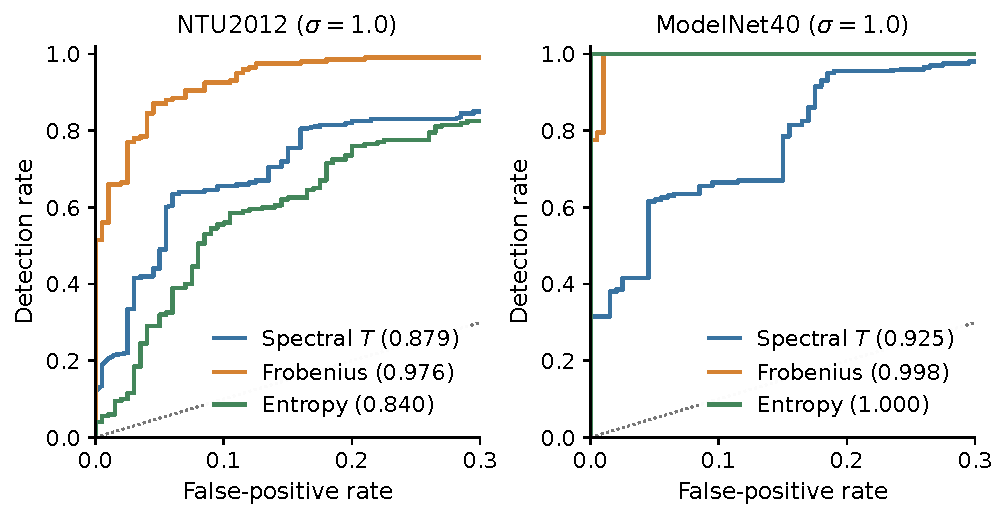
\includegraphics[width=\textwidth]{figures/visual_alarm_roc.pdf}
\caption{Secondary feature-perturbation comparison at $\sigma=1$.
Clean evaluation scores are negatives and paired perturbed scores are
positives. Thresholds are swept on the same evaluation data, so these
ROC curves describe score ranking rather than calibrated deployment
rules. The displayed interval is the low-false-positive-rate portion
of each curve; AUC values refer to the full curve.}
\label{fig:visual-alarm-roc}
\end{figure}

\end{document}
